\documentclass{scrreprt}
\usepackage{listings}
\usepackage{underscore}
\usepackage{graphicx}
\usepackage[bookmarks=true]{hyperref}
\usepackage[utf8]{inputenc}
\usepackage[english]{babel}
\usepackage{float}
\usepackage{enumitem}
\setlist[itemize]{topsep=4pt, itemsep=4pt, parsep=0pt, partopsep=0pt}
\usepackage{pdflscape}
\usepackage{array}
\usepackage{tabularray}

\UseTblrLibrary{booktabs}
\DefTblrTemplate{firsthead,middlehead,lasthead}{default}{}
\DefTblrTemplate{firstfoot}{default}{\UseTblrTemplate{caption}{default}}
\DefTblrTemplate{middlefoot}{default}{\UseTblrTemplate{capcont}{default}}
\DefTblrTemplate{lastfoot}{default}{\UseTblrTemplate{caption}{default}}

\usepackage[
    a4paper,
    left=2cm,
    right=2cm,
    top=3cm,
    bottom=3cm
]{geometry}


\hypersetup{
    bookmarks=false,
    pdftitle={Software Architecture Document},
    pdfauthor={Quach Gia Kiet},
    pdfsubject={SAD for Community Social Network LKForum},
    pdfkeywords={Website, SAD, Software Architecture},
    colorlinks=true,
    linkcolor=blue,
    citecolor=black,
    filecolor=black,
    urlcolor=purple,
    linktoc=page
}%
\def\myversion{1.1}
\date{}

\begin{document}

\begin{flushright}
    \rule{16cm}{5pt}\vskip1cm
    \begin{bfseries}
        \Huge{SOFTWARE ARCHITECTURE \\ DOCUMENT (SAD)}\\
        \vspace{1.5cm}
        for\\
        \vspace{1.5cm}
        LKFORUM WEBSITE\\
        \vspace{1.5cm}
        \LARGE{Version \myversion}\\
        \vspace{1.5cm}
        Prepared by : Quach Gia Kiet\\
        Vo An Khoi\\
        \vspace{1.5cm}
        Submitted to : Nguyen Trinh Dong \\Lecturer\\
        \vspace{1.5cm}
        \today\\
    \end{bfseries}
\end{flushright}

\tableofcontents

\chapter{Documentation Roadmap}

\section{Document Management and Configuration Control Information}
This document serves as the Software Architecture Document (SAD) for the LKForum project. It provides a comprehensive architectural overview of the system, using a number of different architectural views to depict different aspects of the system. 

\section{Purpose and Scope of the SAD}
The purpose of this document is to define and describe the software architecture of the LKForum platform, a community-driven social networking site. The scope includes the backend API (Go/Gin), the frontend SPAs (Svelte), the data storage strategy (MongoDB, Redis), and the deployment environment (Docker). This document is intended to be read by developers, system administrators, and project stakeholders.

\section{How the SAD Is Organized}
This SAD follows the SEI "Views and Beyond" documentation template.
\begin{itemize}
    \item \textbf{Chapter 1:} Documentation Roadmap.
    \item \textbf{Chapter 2:} Architecture Background (Problem and Solution contexts).
    \item \textbf{Chapter 3:} Views (System Context, Module, and Allocation views).
    \item \textbf{Chapter 4:} Relations Among Views.
\end{itemize}

\chapter{Architecture Background}

\section{Problem Background}
\subsection{System Overview}
LKForum is a modern community social networking platform designed to facilitate user engagement, content sharing, and real-time communication. It provides isolated sub-forums (communities) where users can post content, vote, comment, and engage in real-time private messaging.

\subsection{Significant Driving Requirements}
The software architecture was driven by several key Quality Attributes (documented deeply in the Attribute-Driven Design - ADD document):
\begin{itemize}
    \item \textbf{Performance:} High-throughput feed retrieval and real-time WebSocket messaging.
    \item \textbf{Security:} Strong authentication (JWT), RBAC, and End-to-End Encryption (E2EE) for messages.
    \item \textbf{Maintainability:} Strict Layered Architecture to facilitate future feature expansions.
\end{itemize}

\section{Solution Background}
\subsection{Architectural Approaches}
The solution utilizes a \textbf{Client-Server} architectural style combined with an \textbf{Event-Driven} internal approach. 
\begin{itemize}
    \item \textbf{Backend:} A monolithic Go application utilizing the Gin framework for high-performance HTTP routing. It employs a Layered Architecture (Controller $\rightarrow$ Service $\rightarrow$ Repository) to isolate business logic.
    \item \textbf{Frontend:} Separate Single Page Applications (SPAs) built with Svelte for distinct administrative and user boundaries.
    \item \textbf{Asynchronous Processing:} Go Channels are used as an in-memory Event Bus to handle tasks like notifications without blocking main threads.
    \item \textbf{Persistence \& Caching:} MongoDB provides flexible schema design for varying post types, while Redis serves as a Read-Through cache and session store.
\end{itemize}

\chapter{Views}

This section specifies the software architecture using multiple perspectives based on the C4 Model and SEI Viewpoints. Each view is accompanied by an Element Catalog that provides deeper textual descriptions of the components.

\section{Component-and-Connector View (System Context)}
This view illustrates how the system interacts with its environment and external actors at runtime.

\subsection{Primary Presentation}
\begin{figure}[H]
    \centering
    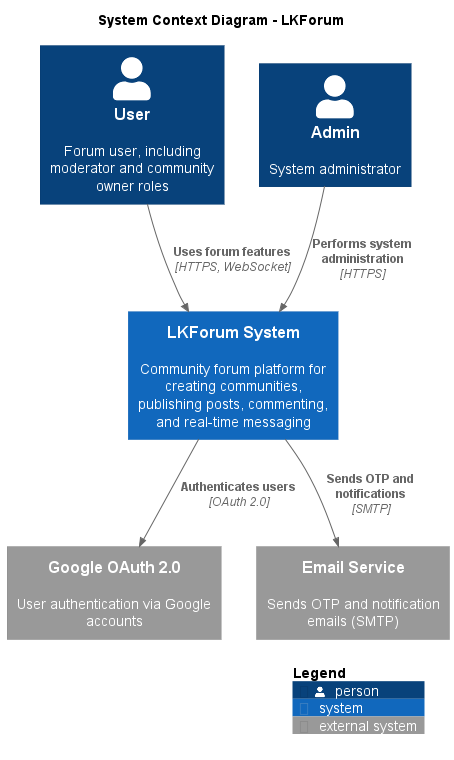
\includegraphics[width=0.9\textwidth]{c4/LKForum_System_Context.png}
    \caption{System Context Diagram}
\end{figure}

\subsection{Element Catalog}
\begin{itemize}
    \item \textbf{Platform User (Actor):} Represents any individual interacting with the LKForum platform. This includes Guests browsing public content, authenticated Members posting content, and Moderators managing communities.
    \item \textbf{System Administrator (Actor):} A specialized user responsible for global platform health, handling site-wide reports, and configuring overarching system parameters.
    \item \textbf{LKForum System (Software System):} The core subject of this architecture. It processes all business logic, serves user interfaces, and maintains the primary state of the social network.
    \item \textbf{Google OAuth (External System):} A third-party Identity Provider used to facilitate Single Sign-On (SSO), allowing users to authenticate without creating local passwords.
    \item \textbf{Cloudinary (External System):} A third-party media management service. It offloads the burden of storing, resizing, and serving static media assets (avatars, post images) from the primary backend.
    \item \textbf{Email Provider (External System):} An SMTP gateway (e.g., SendGrid or AWS SES) used for delivering transactional emails such as OTPs and password resets.
\end{itemize}

\subsection{Behavior: Sequence Diagrams}
This section contains sequence diagrams that describe the exact runtime behavior and interactions between internal and external components for critical use cases.

\subsubsection{UC-01: Sign Up}
\begin{figure}[H]
    \centering
    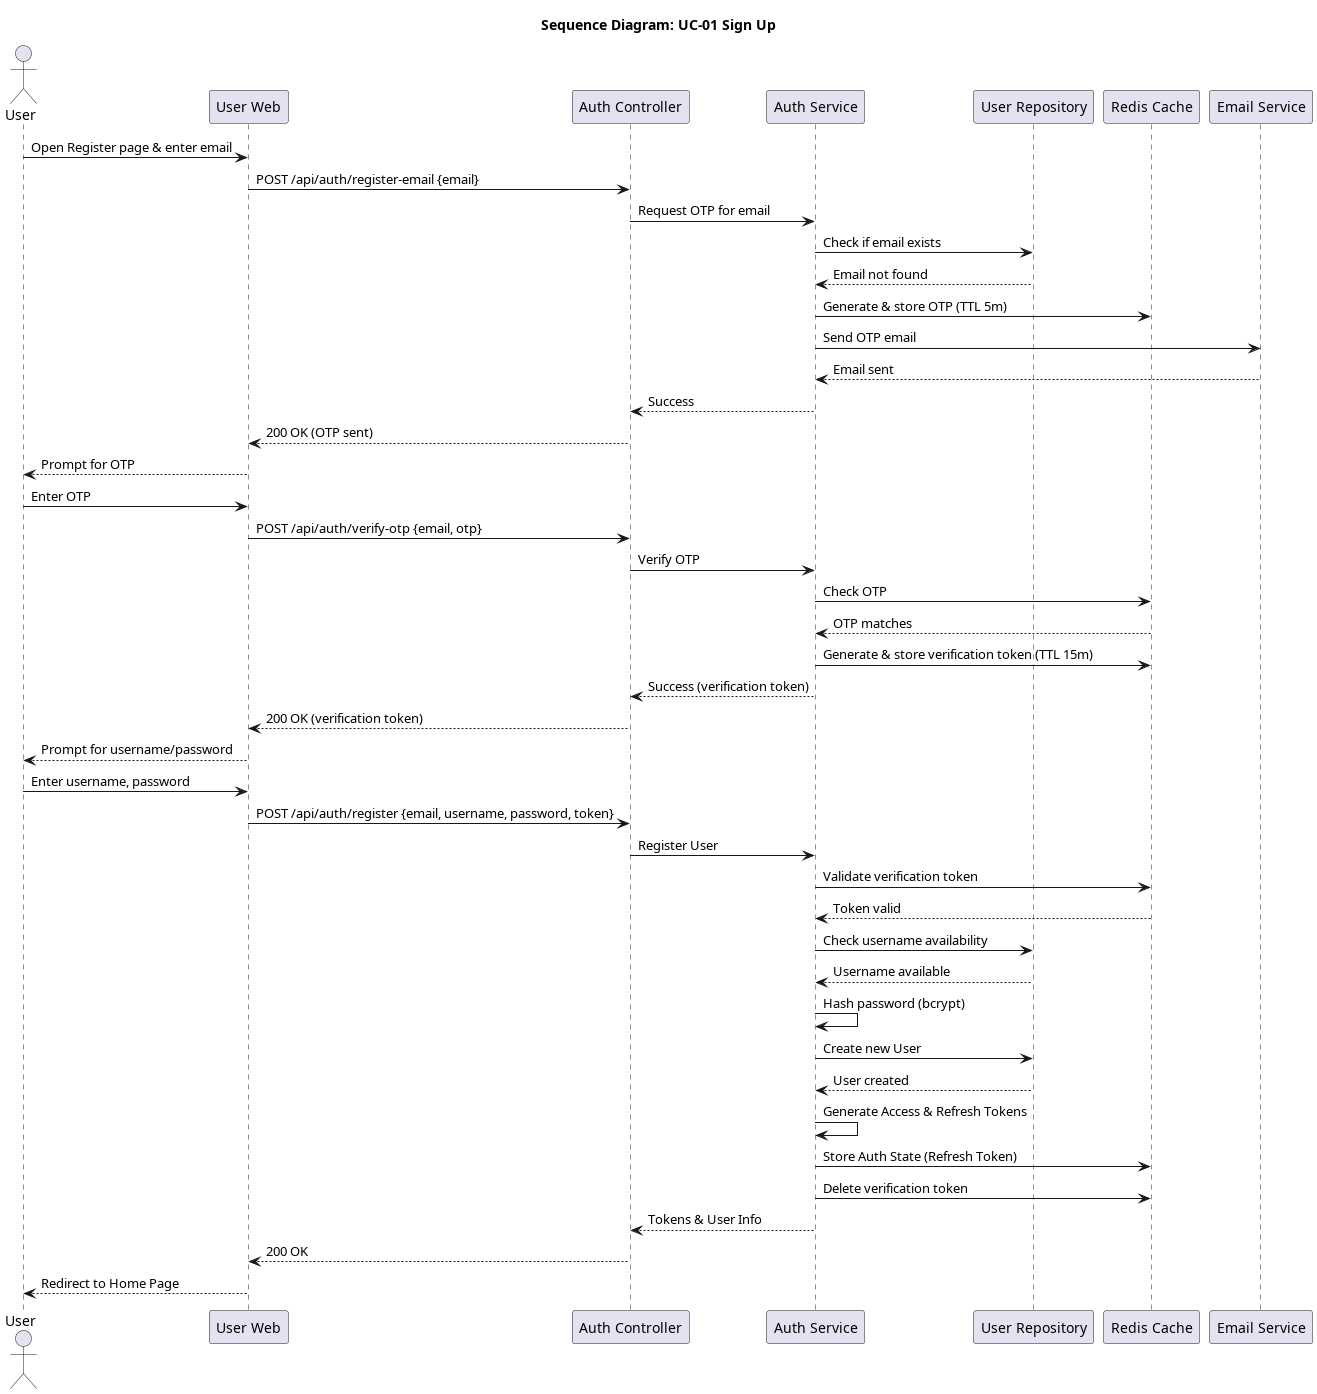
\includegraphics[width=0.9\textwidth]{diagrams/seq_01_sign_up.png}
    \caption{Sequence Diagram for Sign Up}
\end{figure}

\subsubsection{UC-02.1: Local Sign In}
\begin{figure}[H]
    \centering
    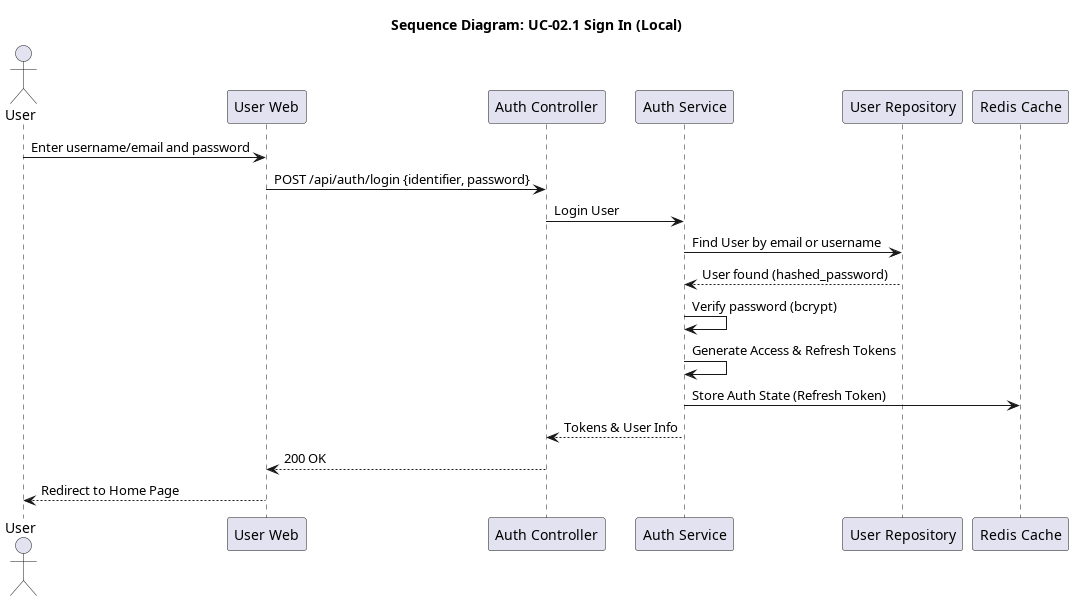
\includegraphics[width=0.9\textwidth]{diagrams/seq_02_local_sign_in.png}
    \caption{Sequence Diagram for Local Sign In}
\end{figure}

\subsubsection{UC-02.2: Google Sign In}
\begin{figure}[H]
    \centering
    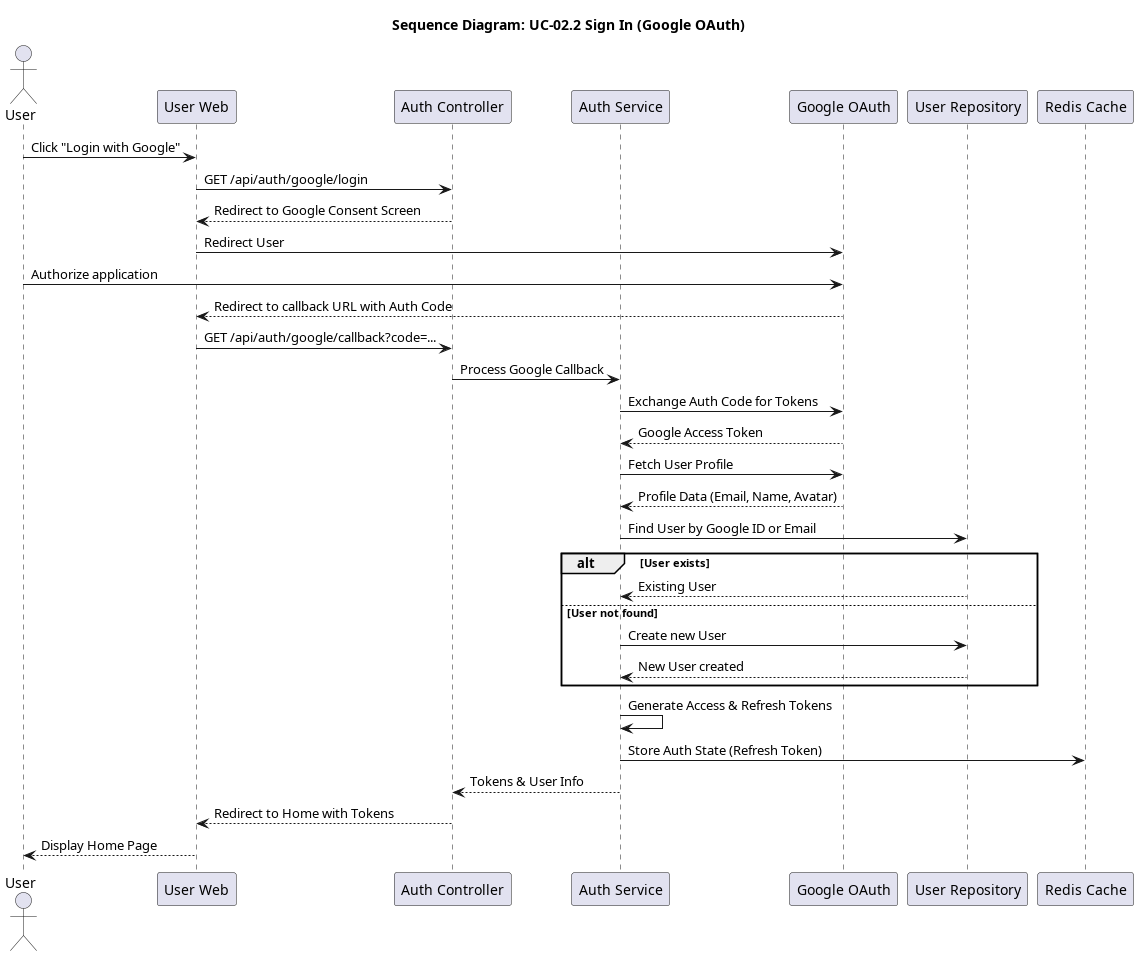
\includegraphics[width=0.9\textwidth]{diagrams/seq_02_google_sign_in.png}
    \caption{Sequence Diagram for Google OAuth Sign In}
\end{figure}

\subsubsection{UC-03: Forgot Password}
\begin{figure}[H]
    \centering
    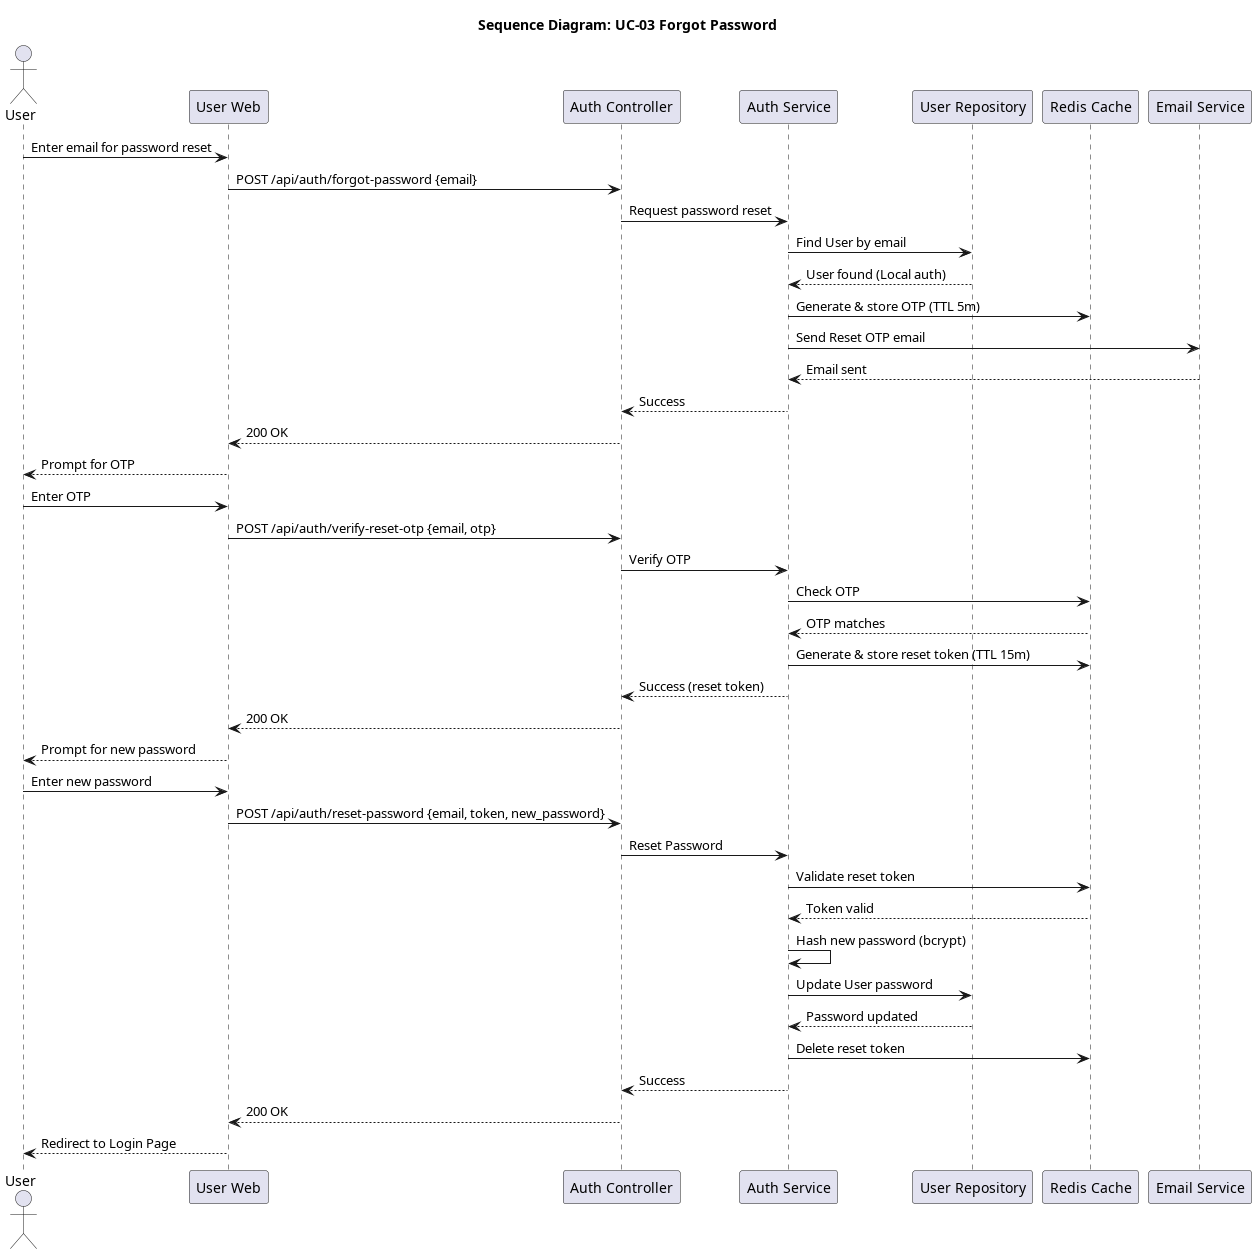
\includegraphics[width=0.9\textwidth]{diagrams/seq_03_forgot_password.png}
    \caption{Sequence Diagram for Forgot Password}
\end{figure}

\subsubsection{UC-04: Manage Profile}
\begin{figure}[H]
    \centering
    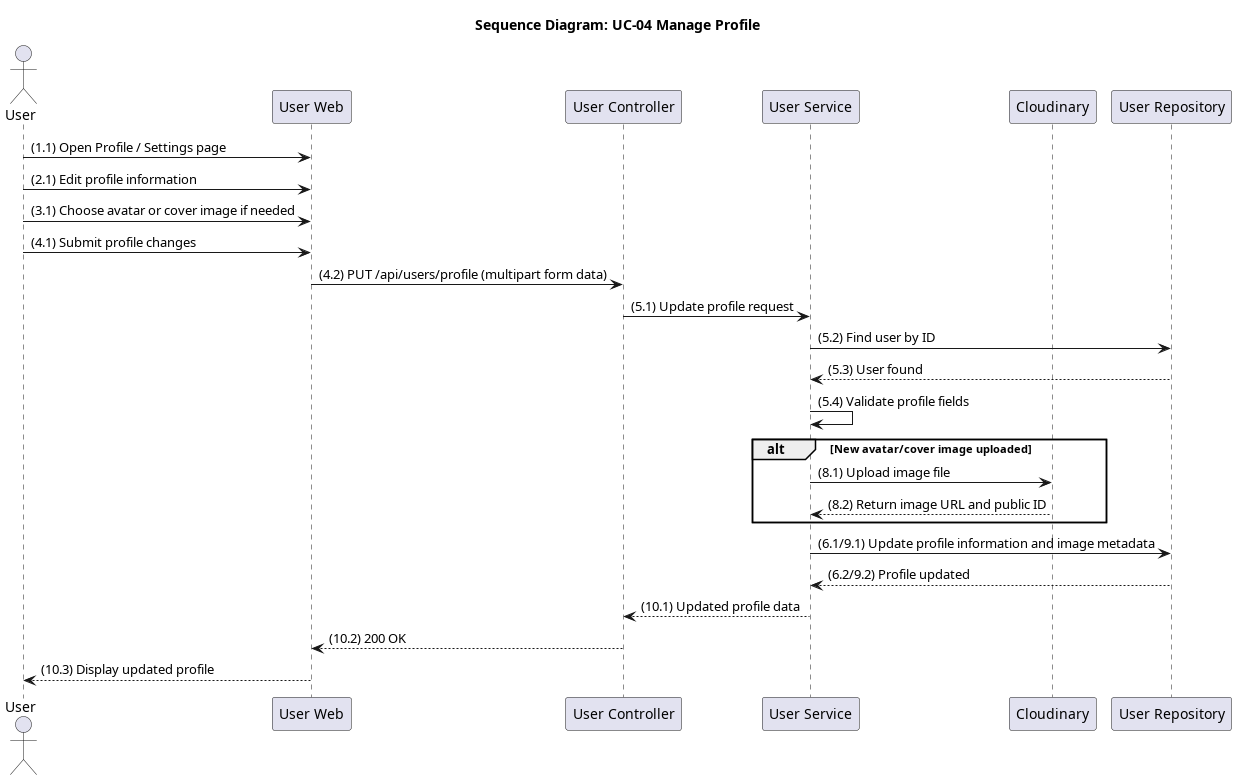
\includegraphics[width=0.9\textwidth]{diagrams/seq_04_manage_profile.png}
    \caption{Sequence Diagram for Manage Profile}
\end{figure}

\subsubsection{UC-05: Change Settings}
\begin{figure}[H]
    \centering
    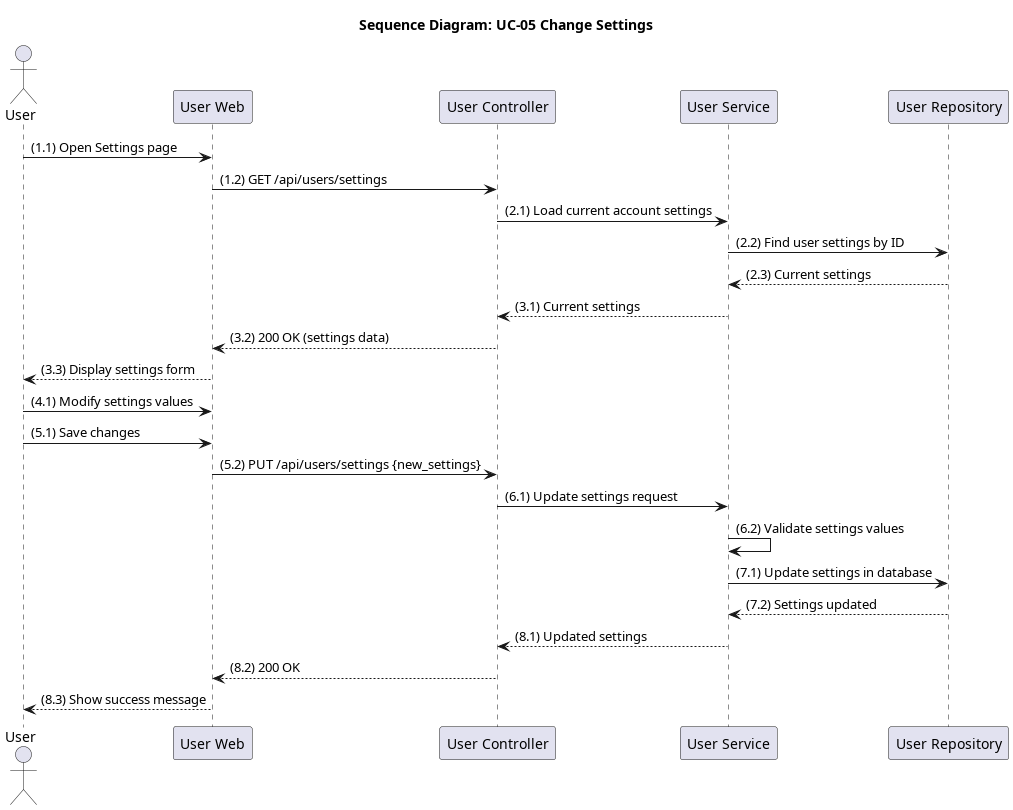
\includegraphics[width=0.9\textwidth]{diagrams/seq_05_change_settings.png}
    \caption{Sequence Diagram for Change Settings}
\end{figure}

\subsubsection{UC-06: View Activity History}
\begin{figure}[H]
    \centering
    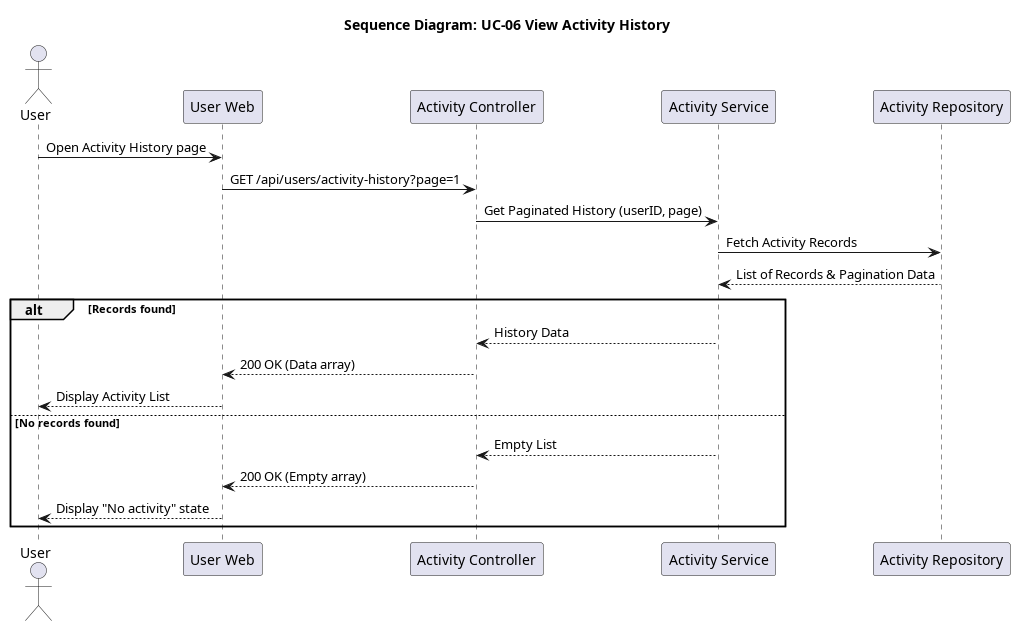
\includegraphics[width=0.9\textwidth]{diagrams/seq_06_view_activity_history.png}
    \caption{Sequence Diagram for View Activity History}
\end{figure}

\subsubsection{UC-07: Follow / Unfollow User}
\begin{figure}[H]
    \centering
    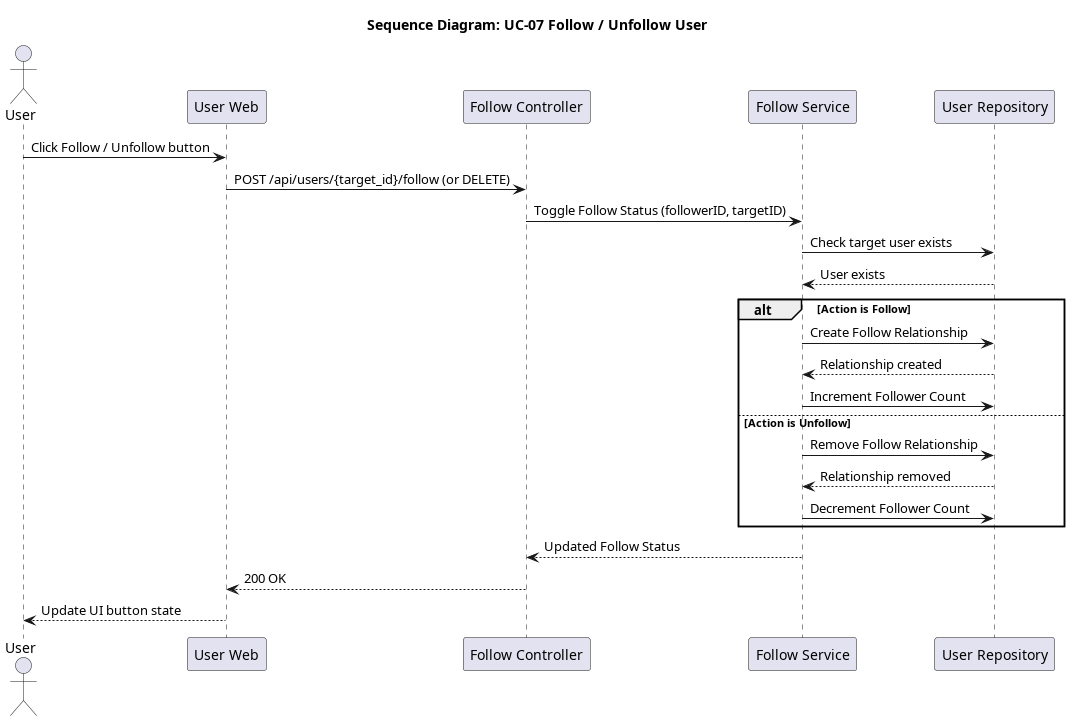
\includegraphics[width=0.9\textwidth]{diagrams/seq_07_follow_unfollow_user.png}
    \caption{Sequence Diagram for Follow / Unfollow User}
\end{figure}

\subsubsection{UC-08: Browse Post}
\begin{figure}[H]
    \centering
    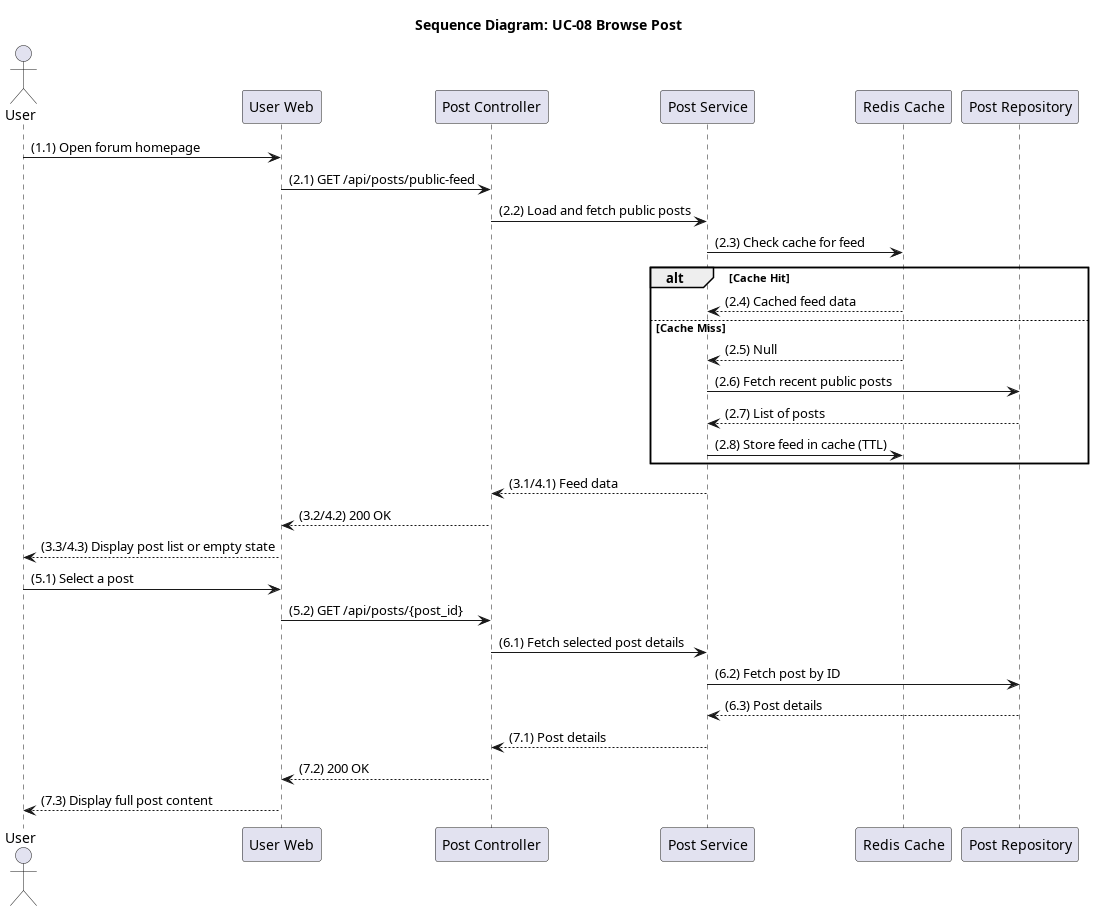
\includegraphics[width=0.9\textwidth]{diagrams/seq_08_browse_post.png}
    \caption{Sequence Diagram for Browse Post}
\end{figure}

\subsubsection{UC-09: Search Content}
\begin{figure}[H]
    \centering
    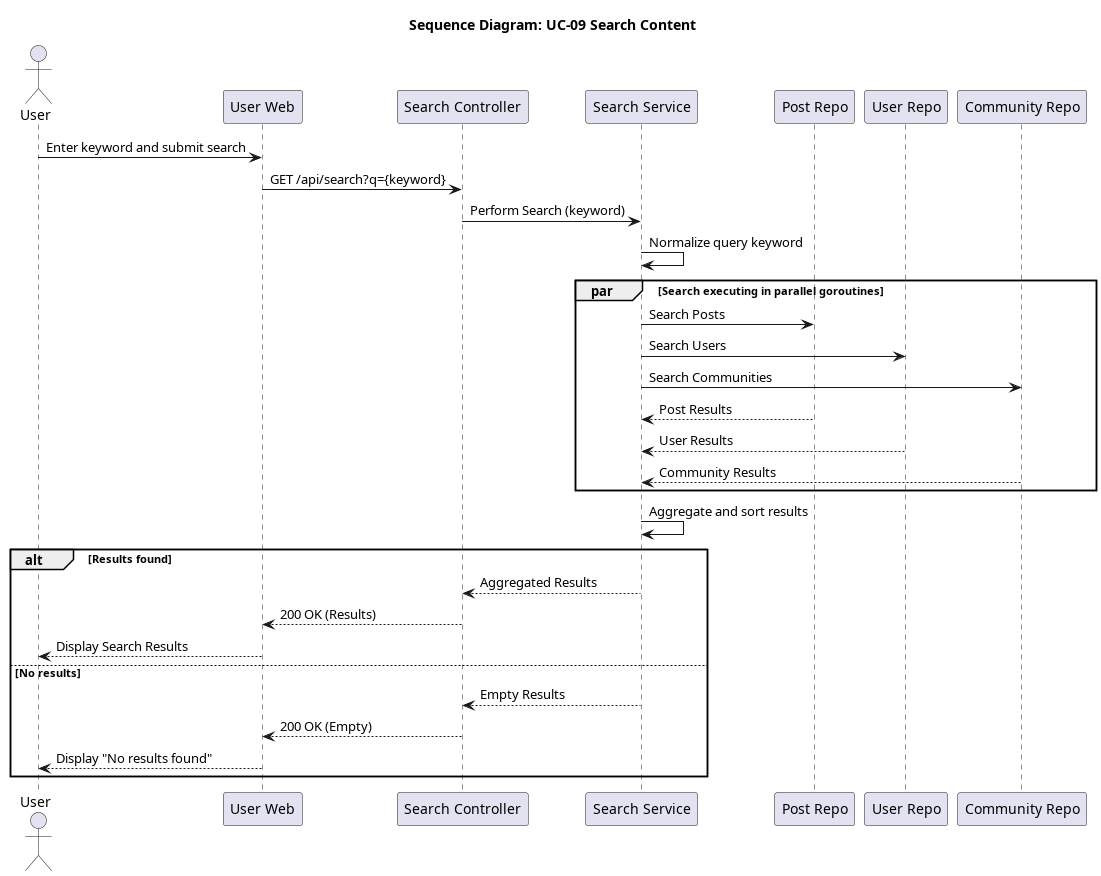
\includegraphics[width=0.9\textwidth]{diagrams/seq_09_search_content.png}
    \caption{Sequence Diagram for Search Content}
\end{figure}

\subsubsection{UC-10: Create Post}
\begin{figure}[H]
    \centering
    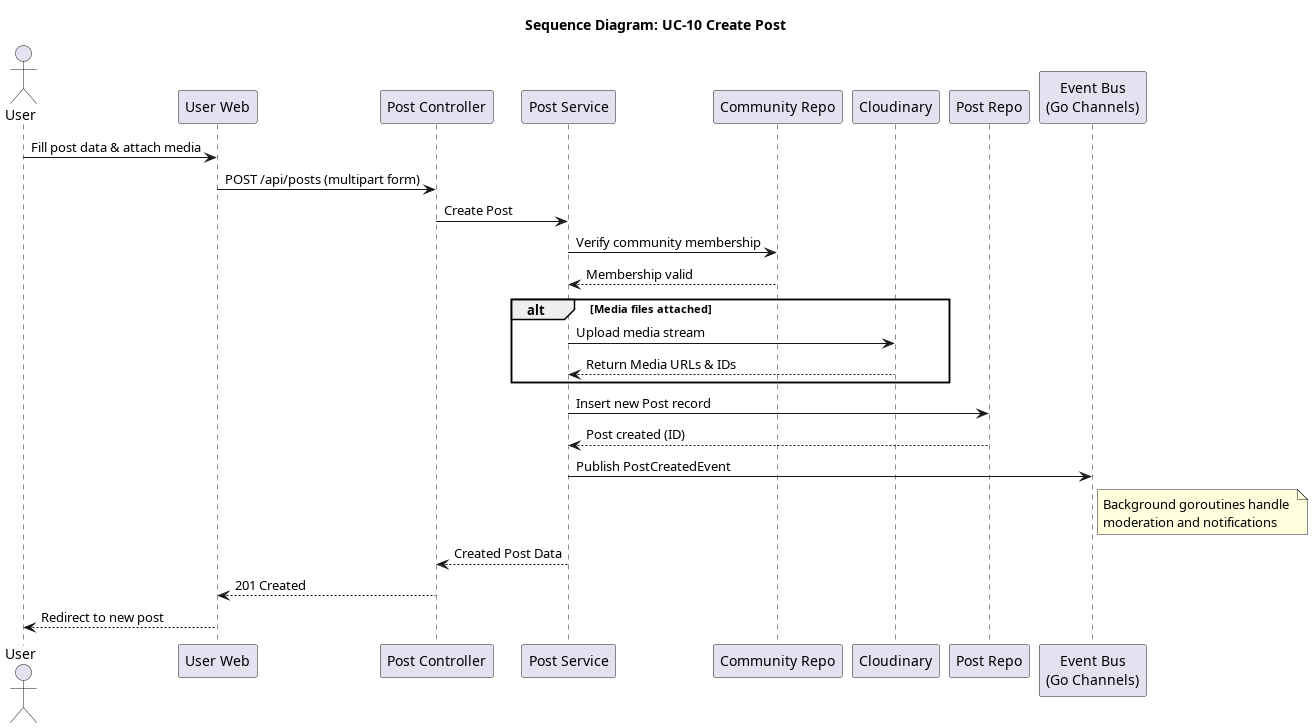
\includegraphics[width=0.9\textwidth]{diagrams/seq_10_create_post.png}
    \caption{Sequence Diagram for Create Post}
\end{figure}

\subsubsection{UC-11: Edit Post}
\begin{figure}[H]
    \centering
    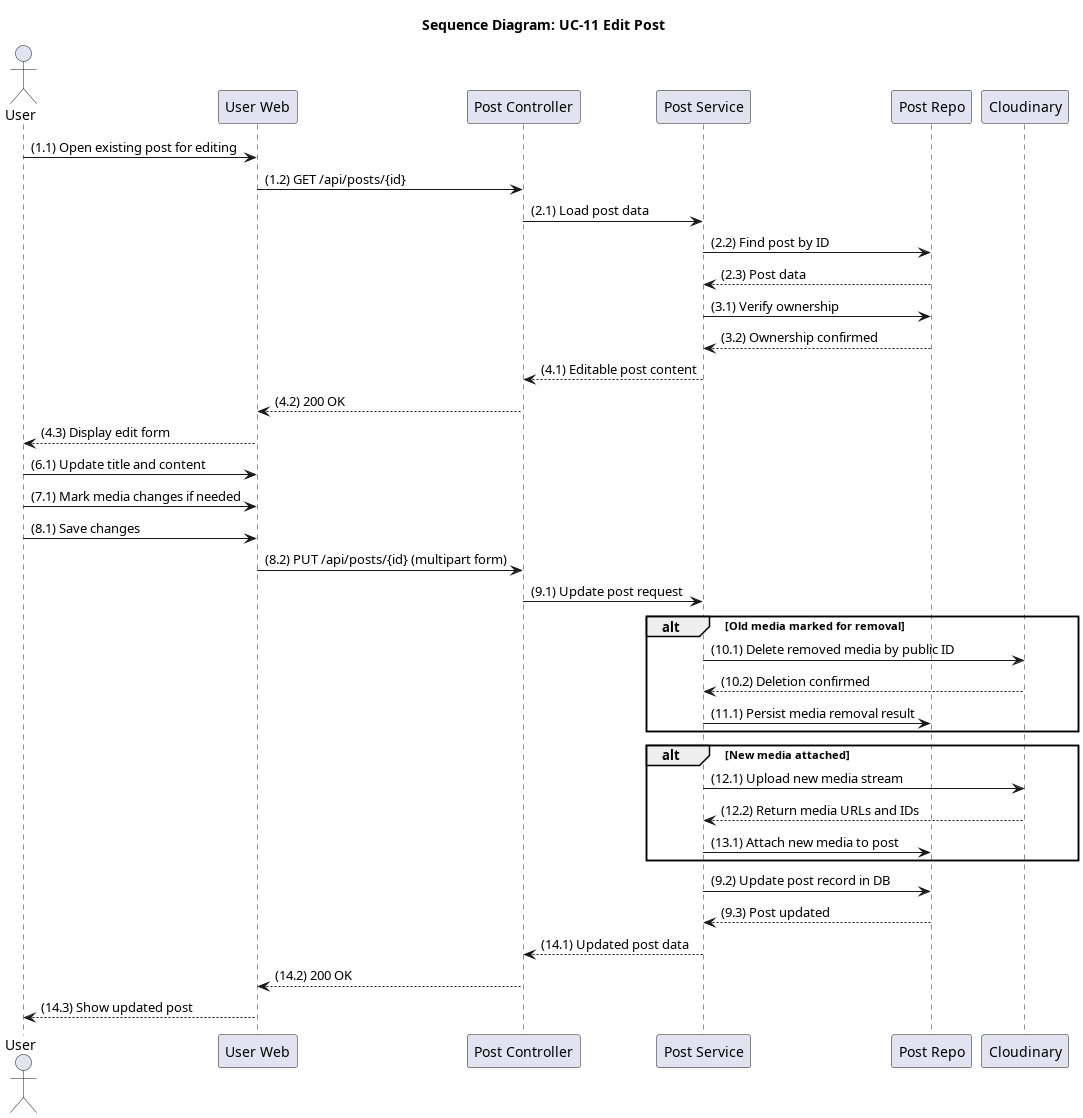
\includegraphics[width=0.9\textwidth]{diagrams/seq_11_edit_post.png}
    \caption{Sequence Diagram for Edit Post}
\end{figure}

\subsubsection{UC-12: Delete Post}
\begin{figure}[H]
    \centering
    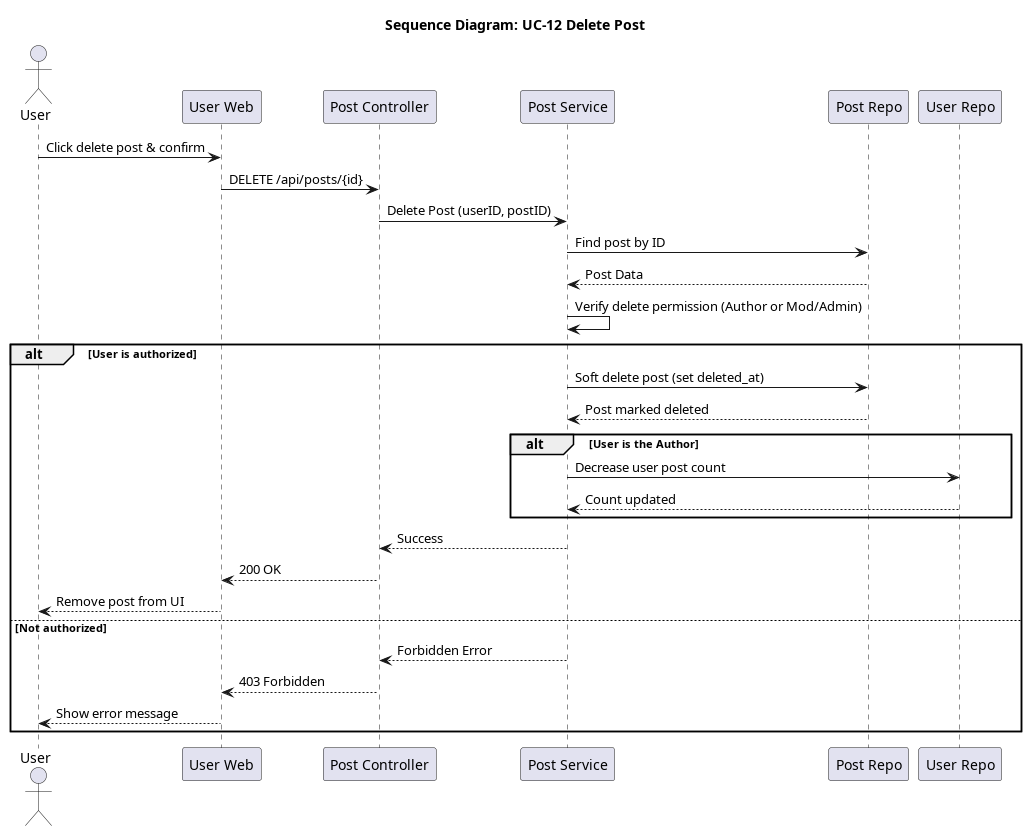
\includegraphics[width=0.9\textwidth]{diagrams/seq_12_delete_post.png}
    \caption{Sequence Diagram for Delete Post}
\end{figure}

\subsubsection{UC-13: Post Comment}
\begin{figure}[H]
    \centering
    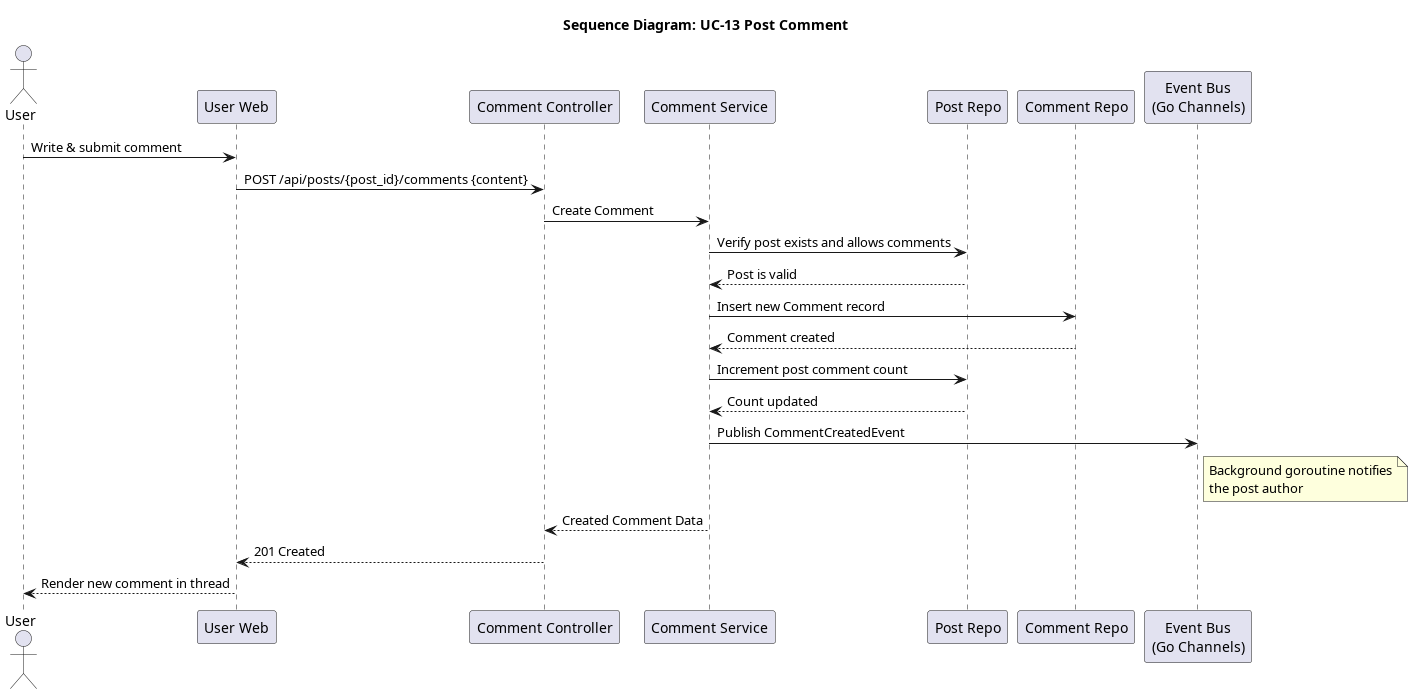
\includegraphics[width=0.9\textwidth]{diagrams/seq_13_post_comment.png}
    \caption{Sequence Diagram for Post Comment}
\end{figure}

\subsubsection{UC-14: Reply to Comment}
\begin{figure}[H]
    \centering
    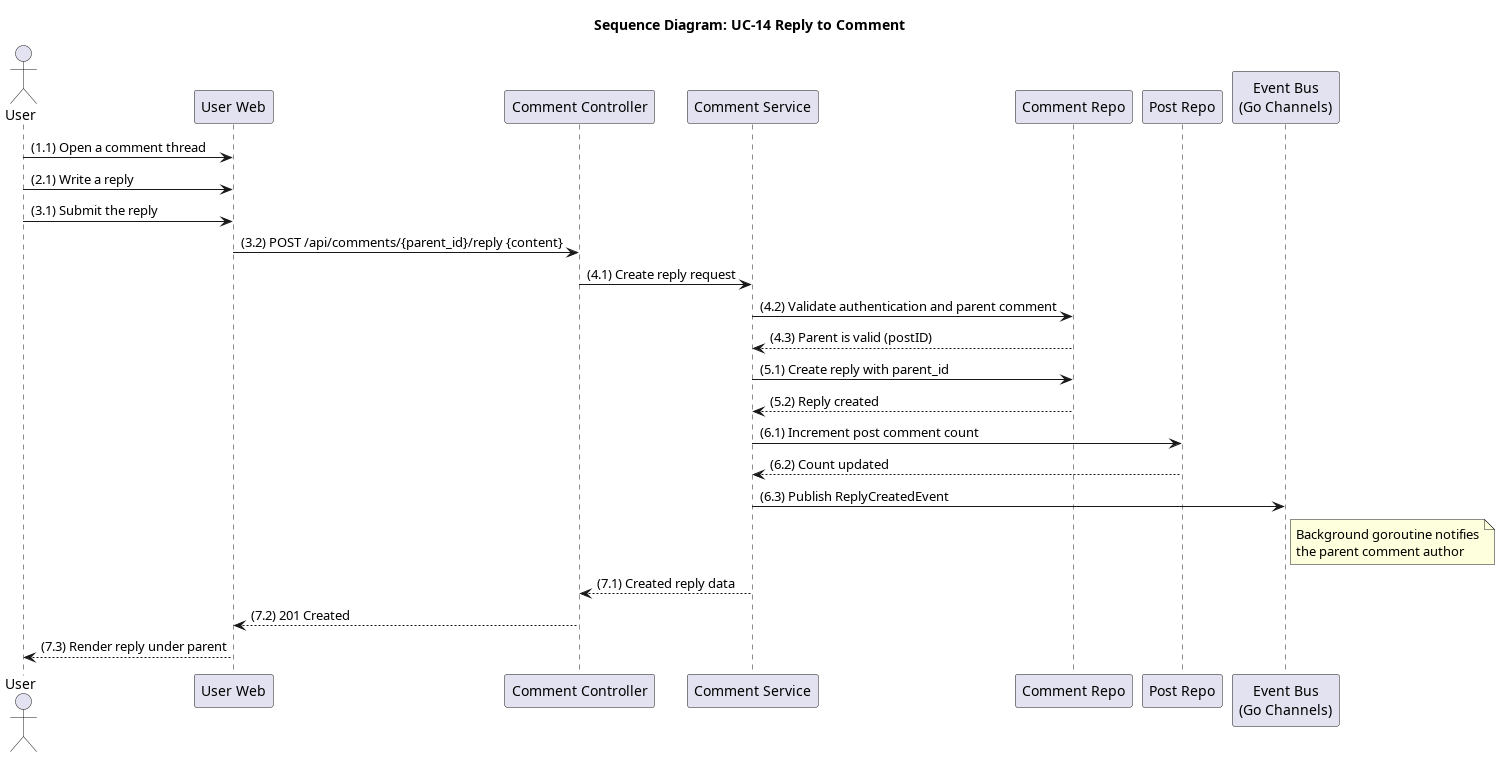
\includegraphics[width=0.9\textwidth]{diagrams/seq_14_reply_to_comment.png}
    \caption{Sequence Diagram for Reply to Comment}
\end{figure}

\subsubsection{UC-15: Vote on Content}
\begin{figure}[H]
    \centering
    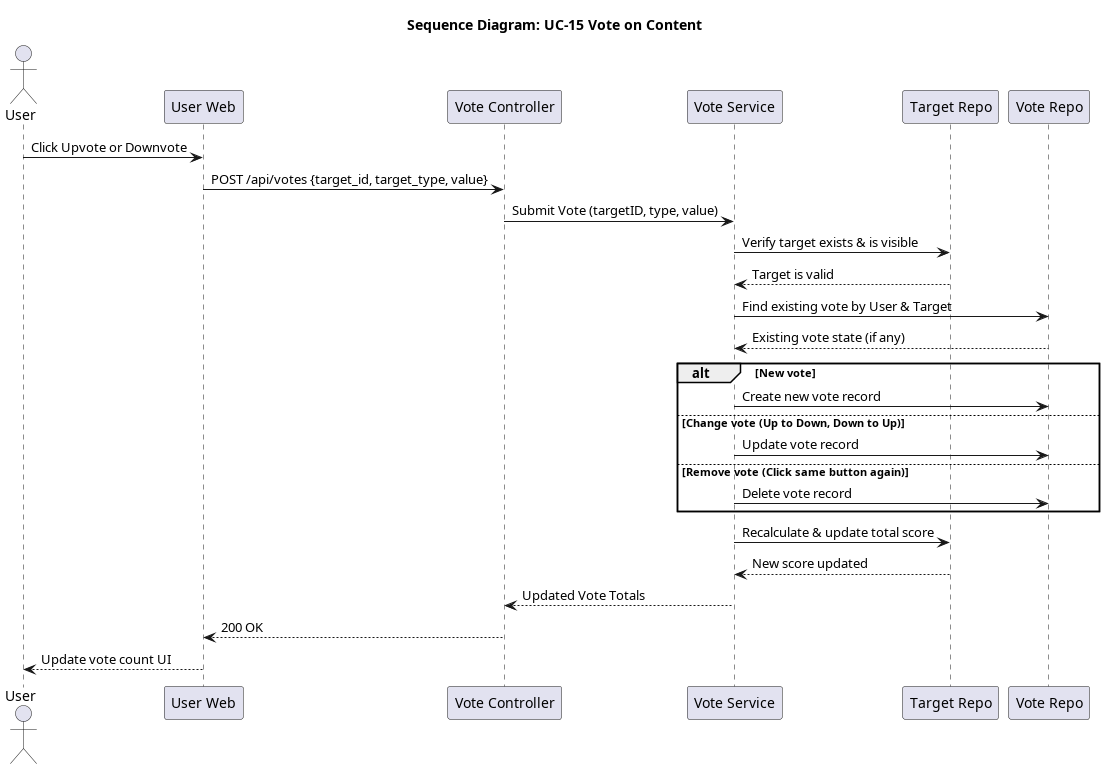
\includegraphics[width=0.9\textwidth]{diagrams/seq_15_vote_on_content.png}
    \caption{Sequence Diagram for Vote on Content}
\end{figure}

\subsubsection{UC-16: Participate in Poll}
\begin{figure}[H]
    \centering
    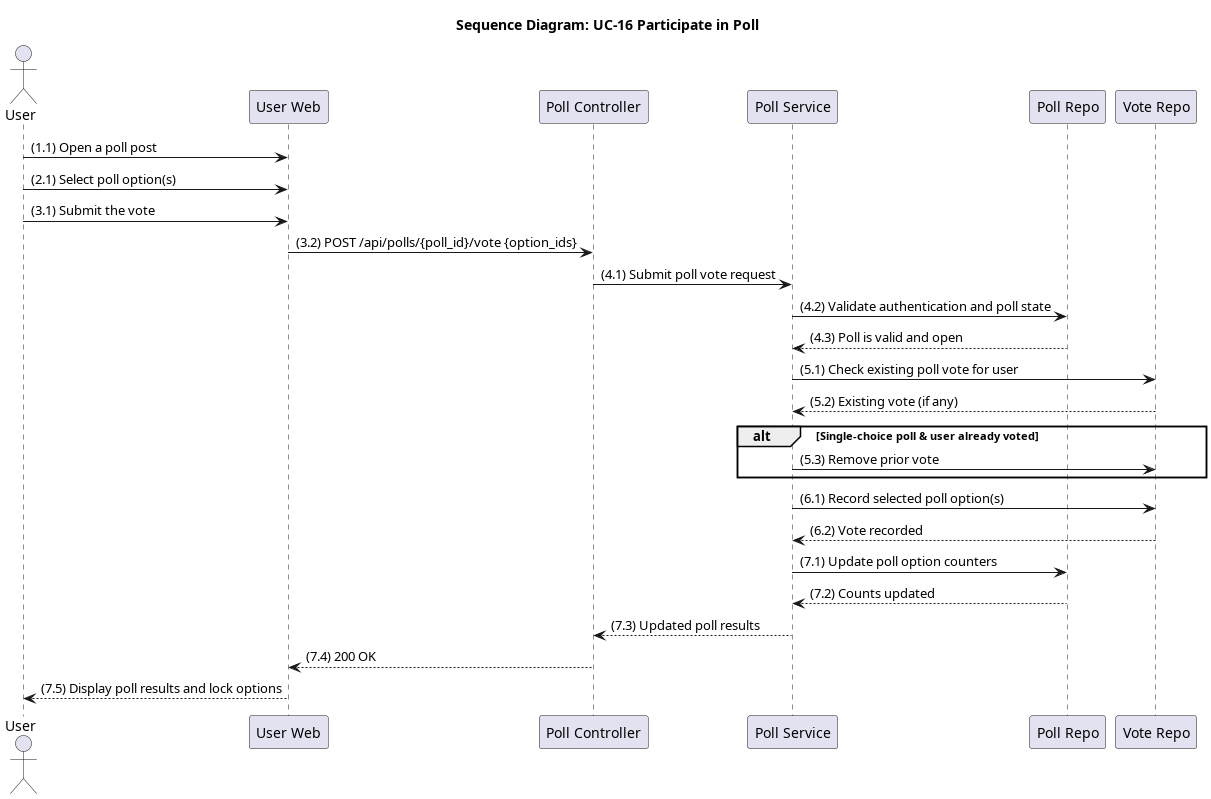
\includegraphics[width=0.9\textwidth]{diagrams/seq_16_participate_in_poll.png}
    \caption{Sequence Diagram for Participate in Poll}
\end{figure}

\subsubsection{UC-17: Save Post}
\begin{figure}[H]
    \centering
    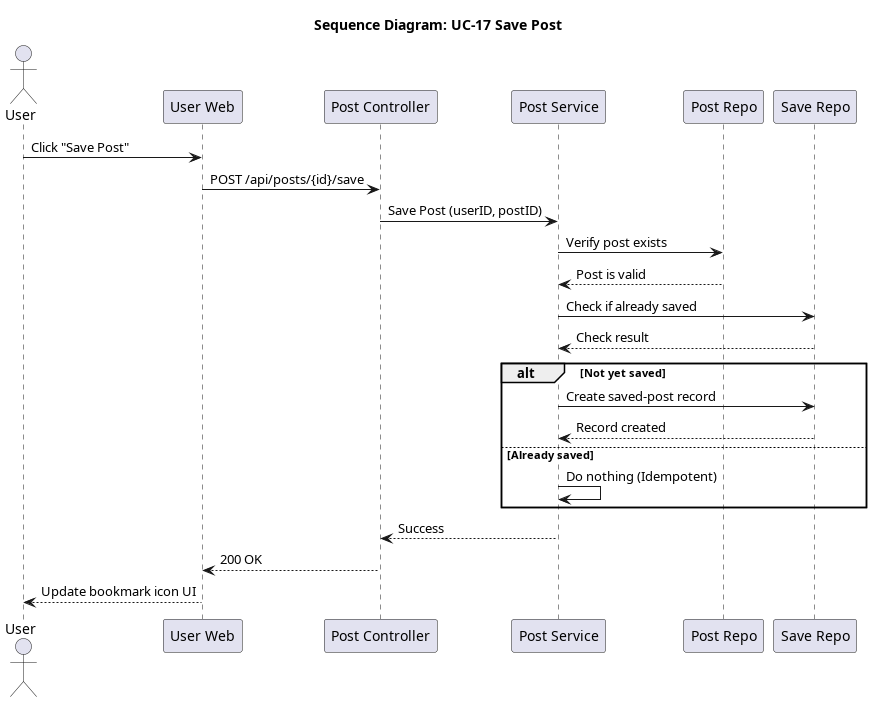
\includegraphics[width=0.9\textwidth]{diagrams/seq_17_save_post.png}
    \caption{Sequence Diagram for Save Post}
\end{figure}

\subsubsection{UC-18: Hide Post}
\begin{figure}[H]
    \centering
    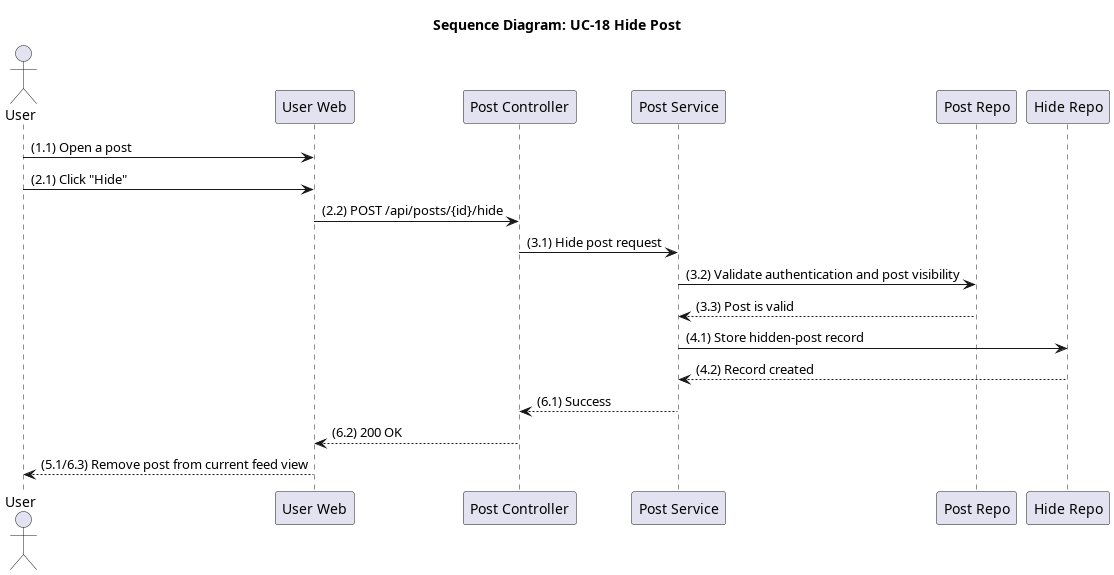
\includegraphics[width=0.9\textwidth]{diagrams/seq_18_hide_post.png}
    \caption{Sequence Diagram for Hide Post}
\end{figure}

\subsubsection{UC-19: Manage Drafts}
\begin{figure}[H]
    \centering
    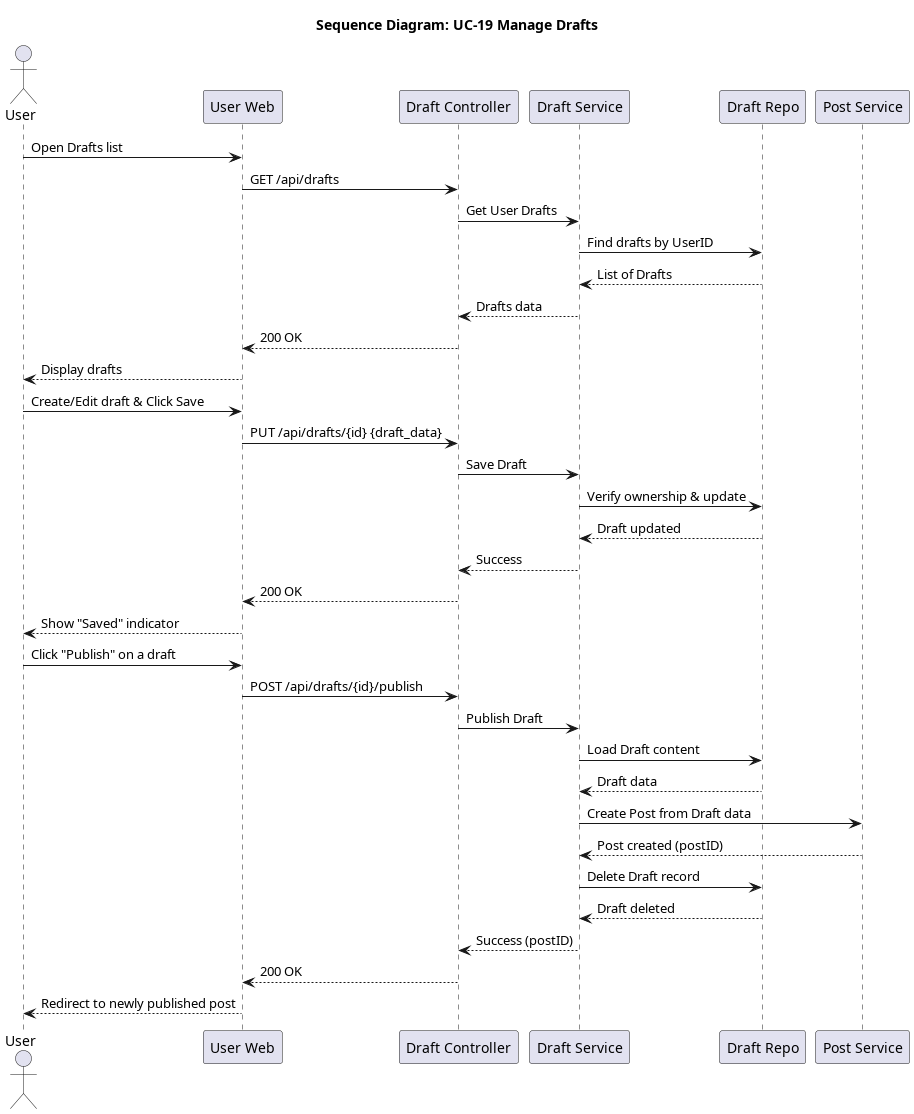
\includegraphics[width=0.9\textwidth]{diagrams/seq_19_manage_drafts.png}
    \caption{Sequence Diagram for Manage Drafts}
\end{figure}

\subsubsection{UC-20: Private Messaging}
\begin{figure}[H]
    \centering
    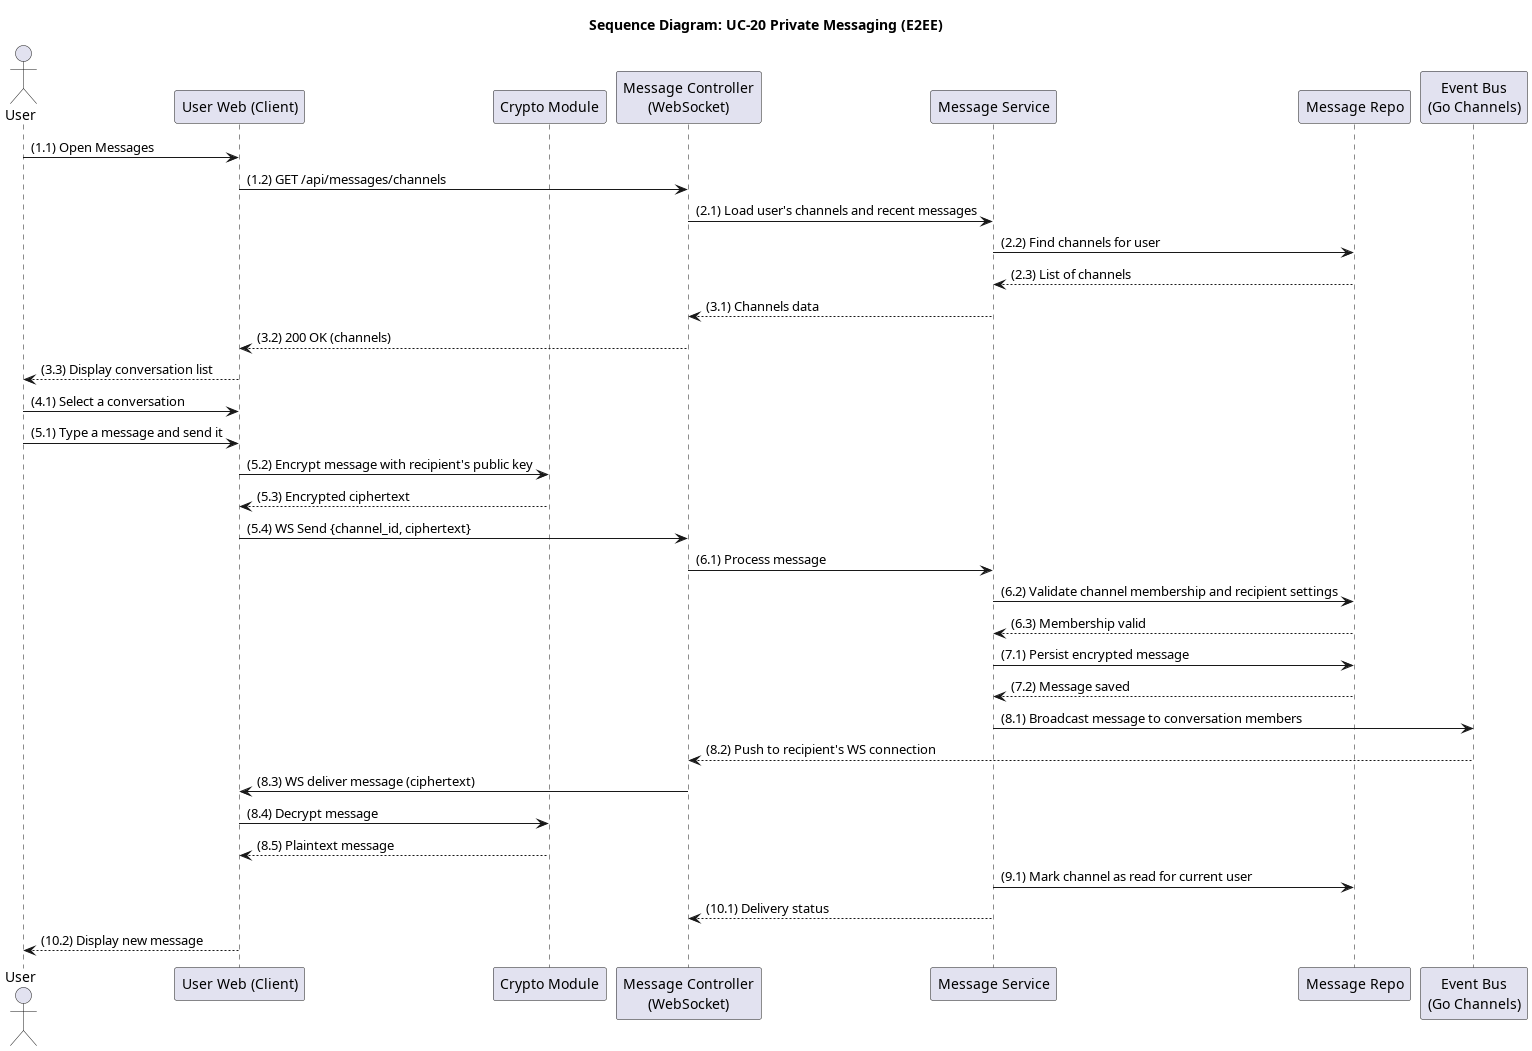
\includegraphics[width=0.9\textwidth]{diagrams/seq_20_private_messaging.png}
    \caption{Sequence Diagram for Private Messaging}
\end{figure}

\subsubsection{UC-21: Manage Notifications}
\begin{figure}[H]
    \centering
    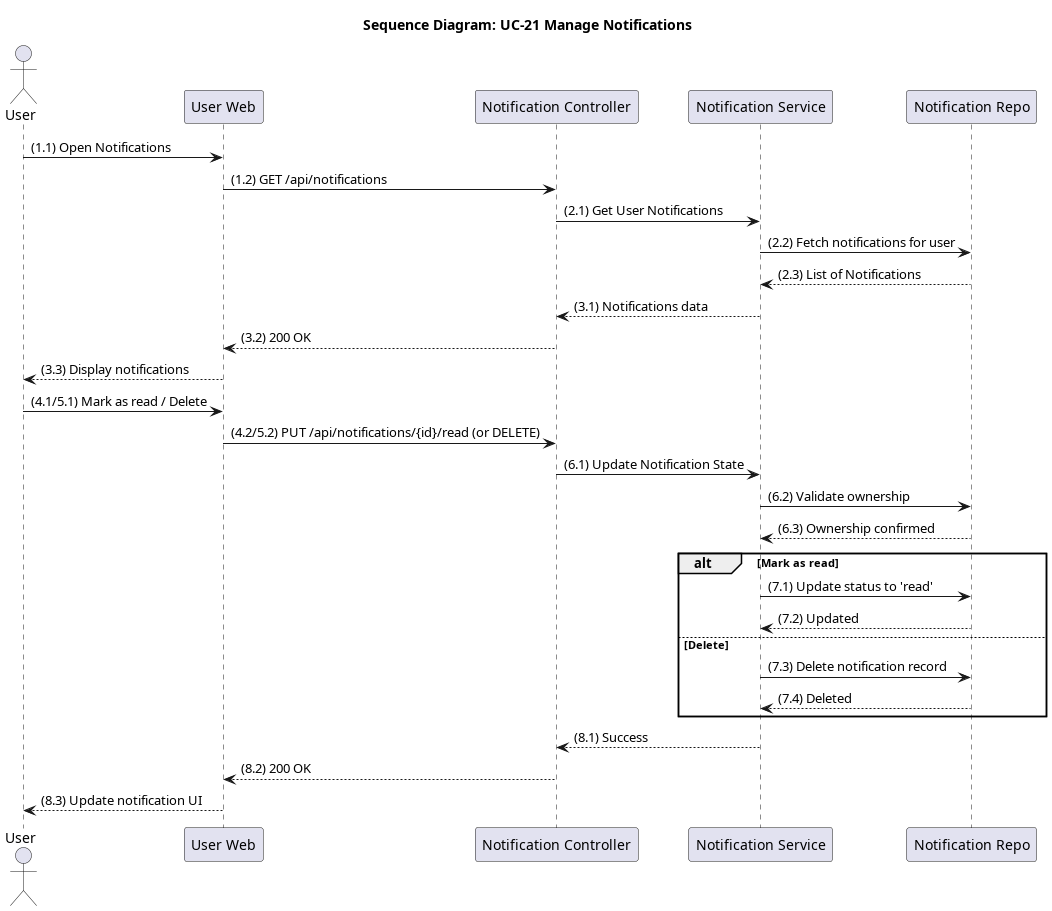
\includegraphics[width=0.9\textwidth]{diagrams/seq_21_manage_notifications.png}
    \caption{Sequence Diagram for Manage Notifications}
\end{figure}

\subsubsection{UC-22: Report Violation}
\begin{figure}[H]
    \centering
    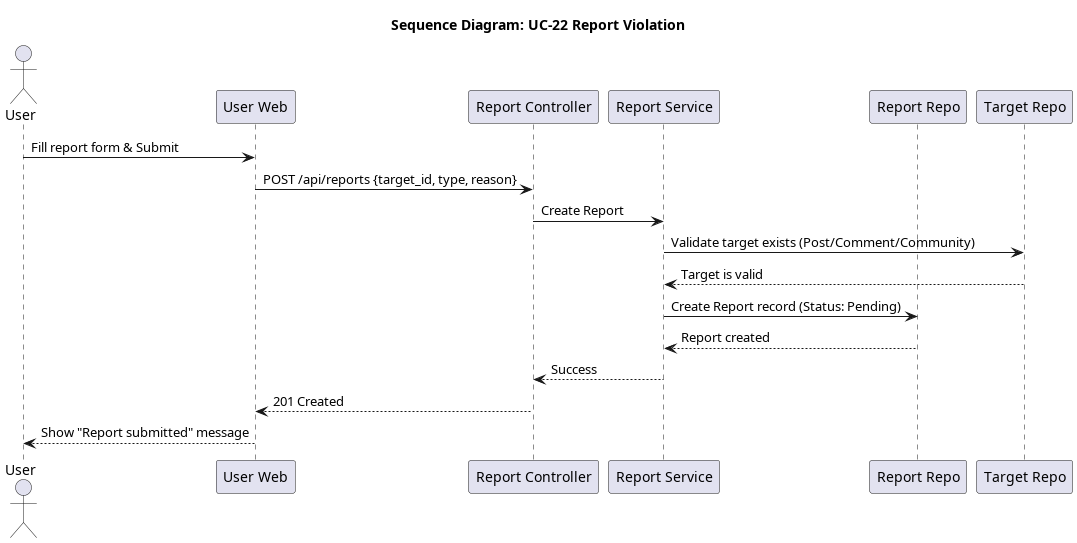
\includegraphics[width=0.9\textwidth]{diagrams/seq_22_report_violation.png}
    \caption{Sequence Diagram for Report Violation}
\end{figure}

\subsubsection{UC-23: Create Community}
\begin{figure}[H]
    \centering
    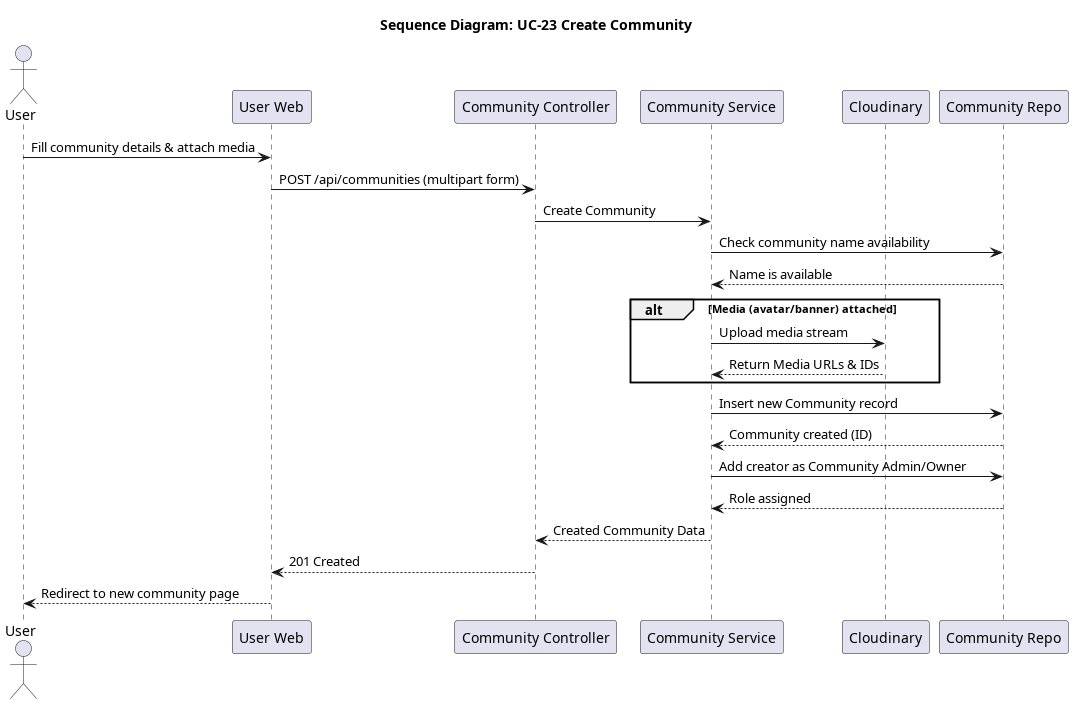
\includegraphics[width=0.9\textwidth]{diagrams/seq_23_create_community.png}
    \caption{Sequence Diagram for Create Community}
\end{figure}

\subsubsection{UC-24: Approve / Reject Post}
\begin{figure}[H]
    \centering
    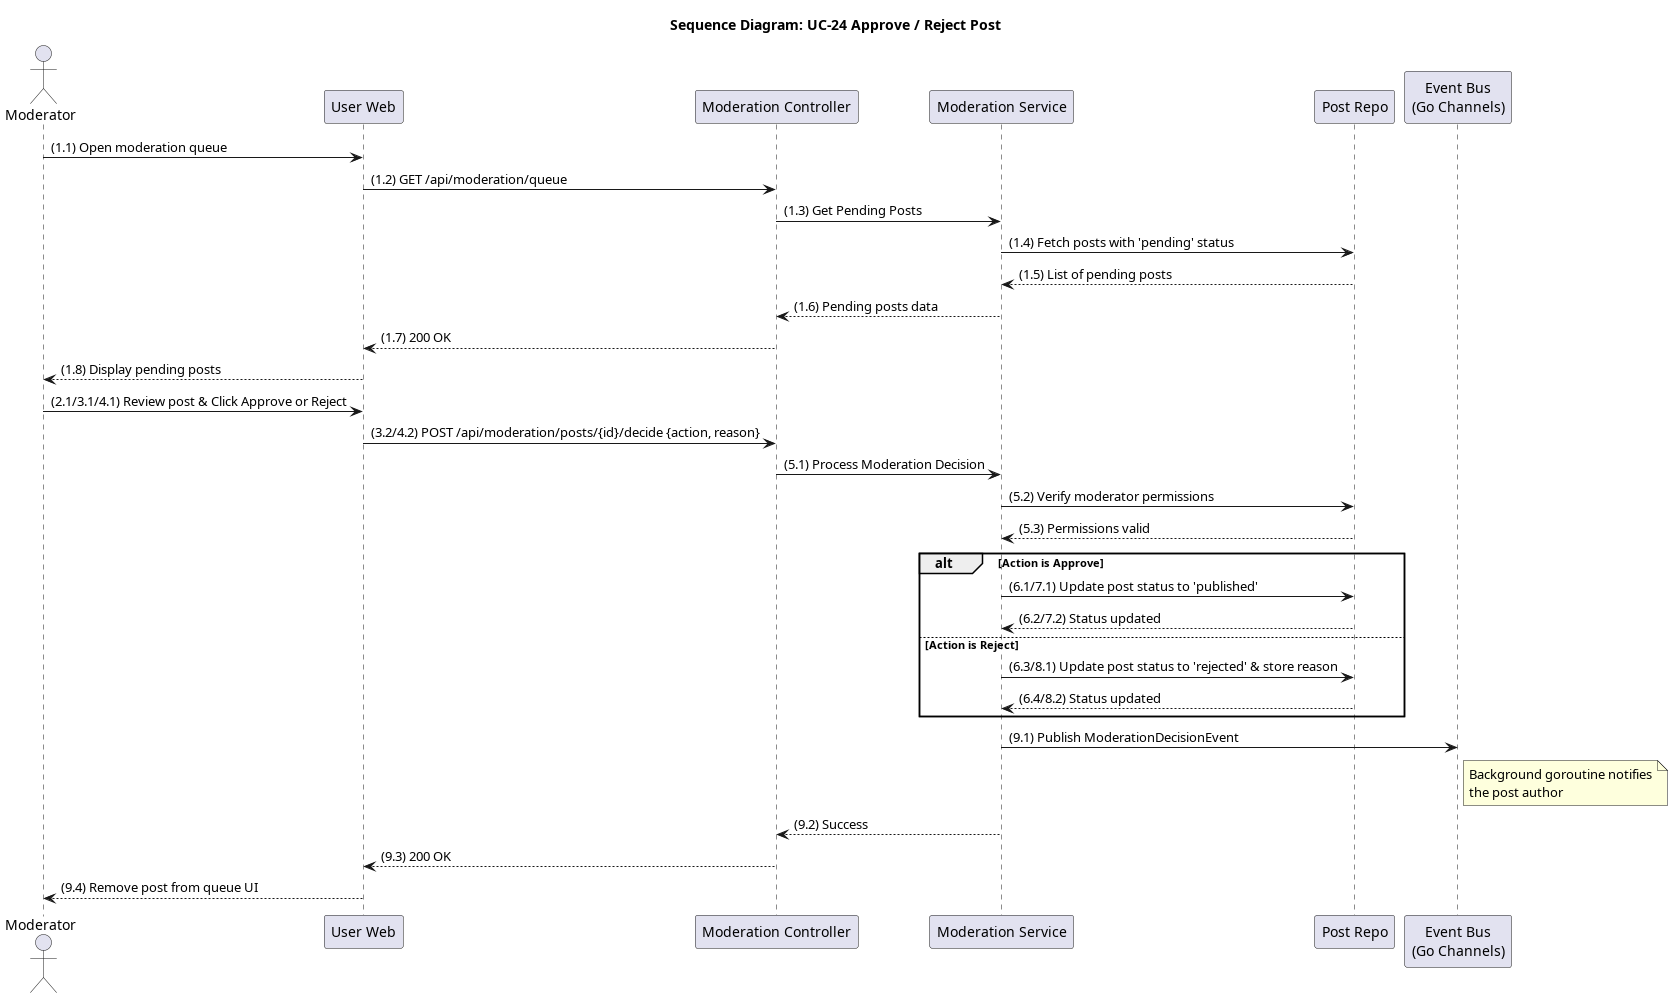
\includegraphics[width=0.9\textwidth]{diagrams/seq_24_approve_reject_post.png}
    \caption{Sequence Diagram for Approve / Reject Post}
\end{figure}

\subsubsection{UC-25: Ban / Mute User}
\begin{figure}[H]
    \centering
    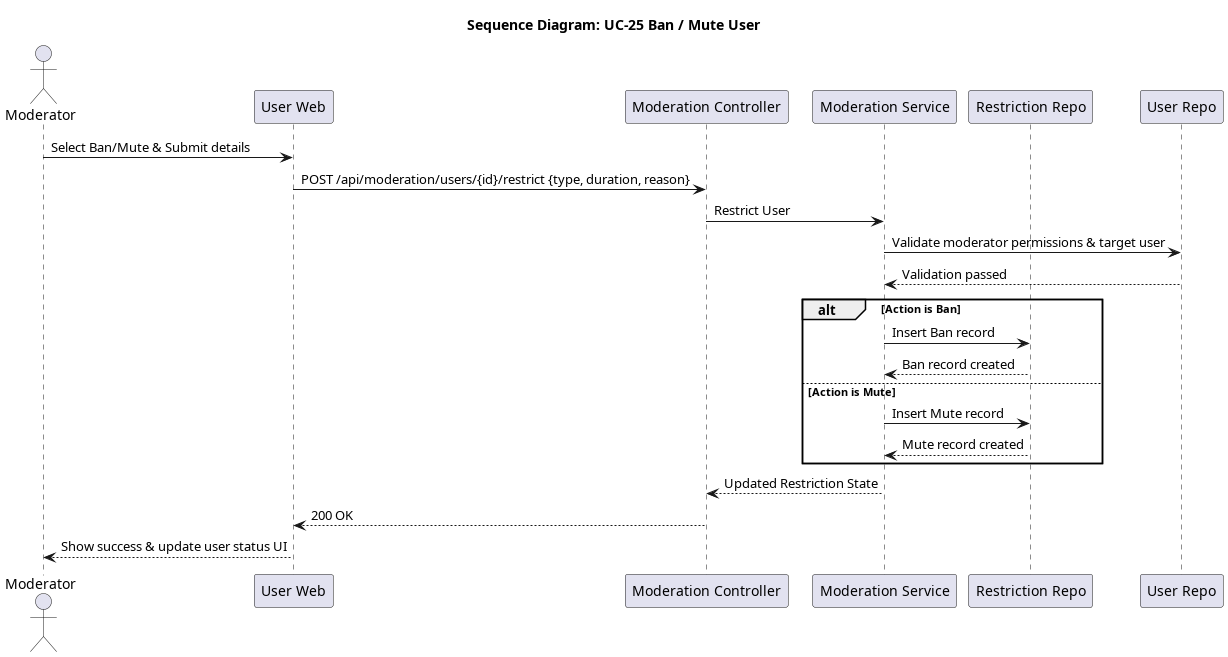
\includegraphics[width=0.9\textwidth]{diagrams/seq_25_ban_mute_user.png}
    \caption{Sequence Diagram for Ban / Mute User}
\end{figure}

\subsubsection{UC-26: Configure Community}
\begin{figure}[H]
    \centering
    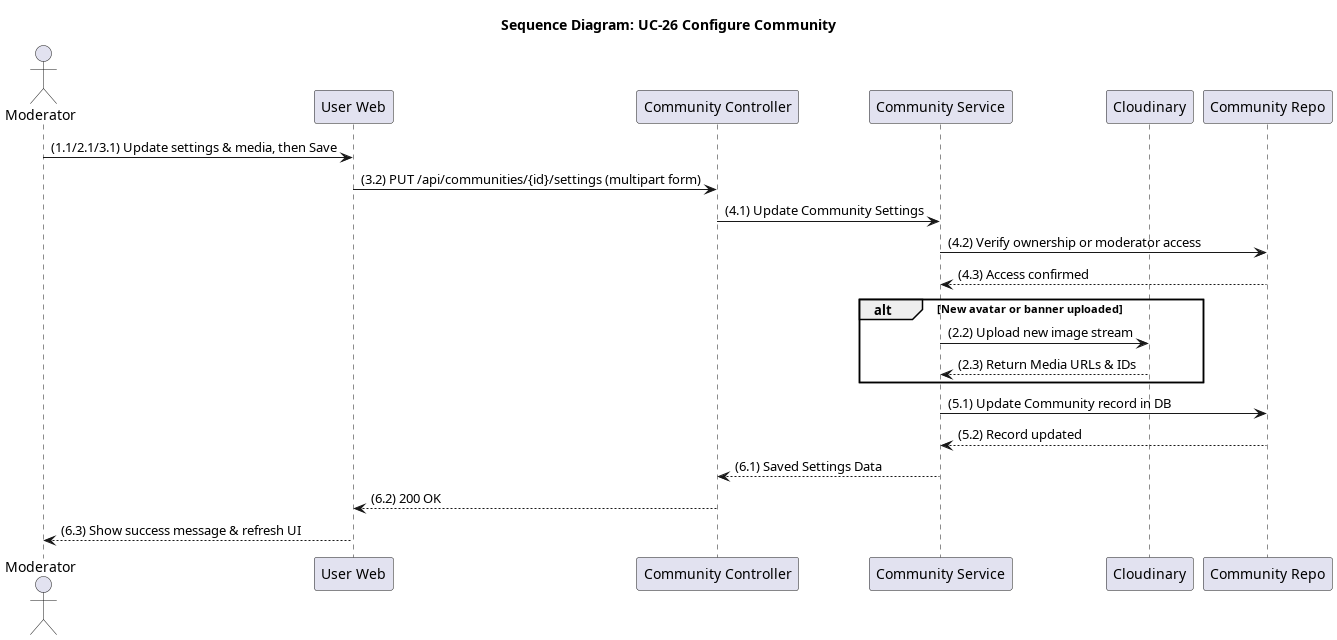
\includegraphics[width=0.9\textwidth]{diagrams/seq_26_configure_community.png}
    \caption{Sequence Diagram for Configure Community}
\end{figure}

\subsubsection{UC-27: Assign Roles}
\begin{figure}[H]
    \centering
    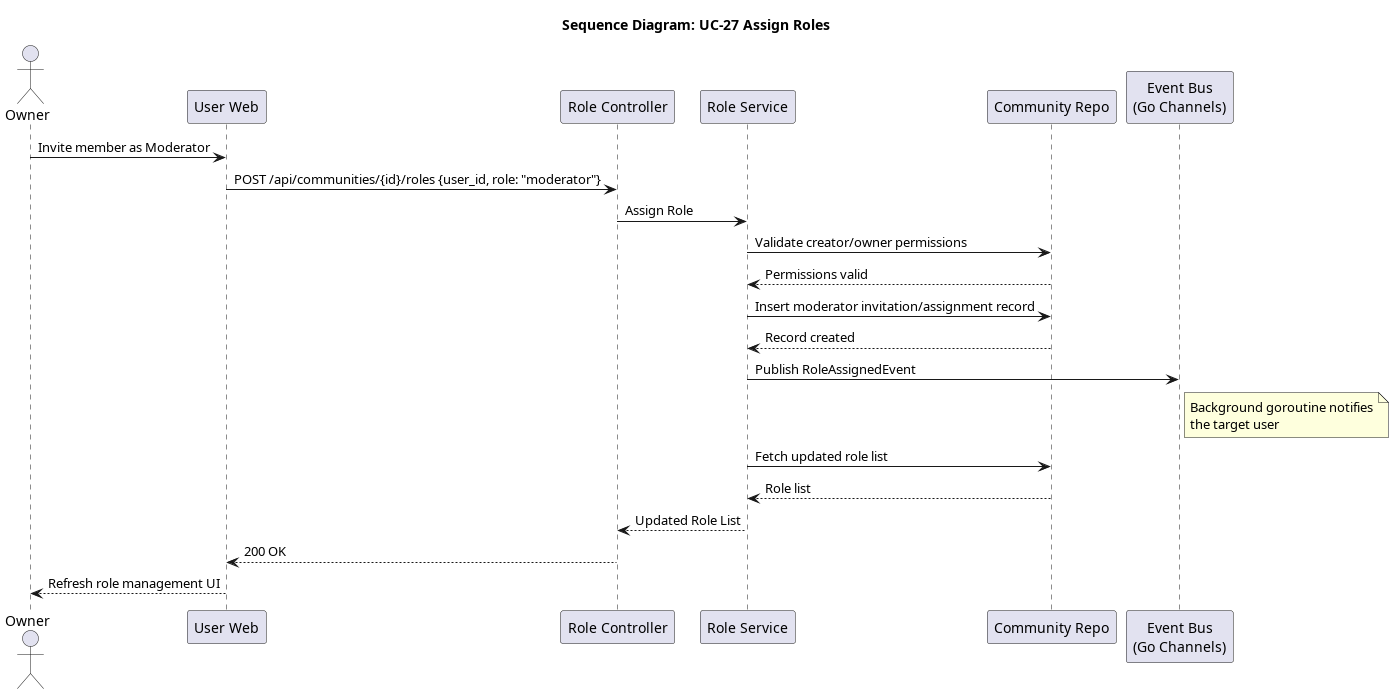
\includegraphics[width=0.9\textwidth]{diagrams/seq_27_assign_roles.png}
    \caption{Sequence Diagram for Assign Roles}
\end{figure}

\subsubsection{UC-28: Handle Global Reports}
\begin{figure}[H]
    \centering
    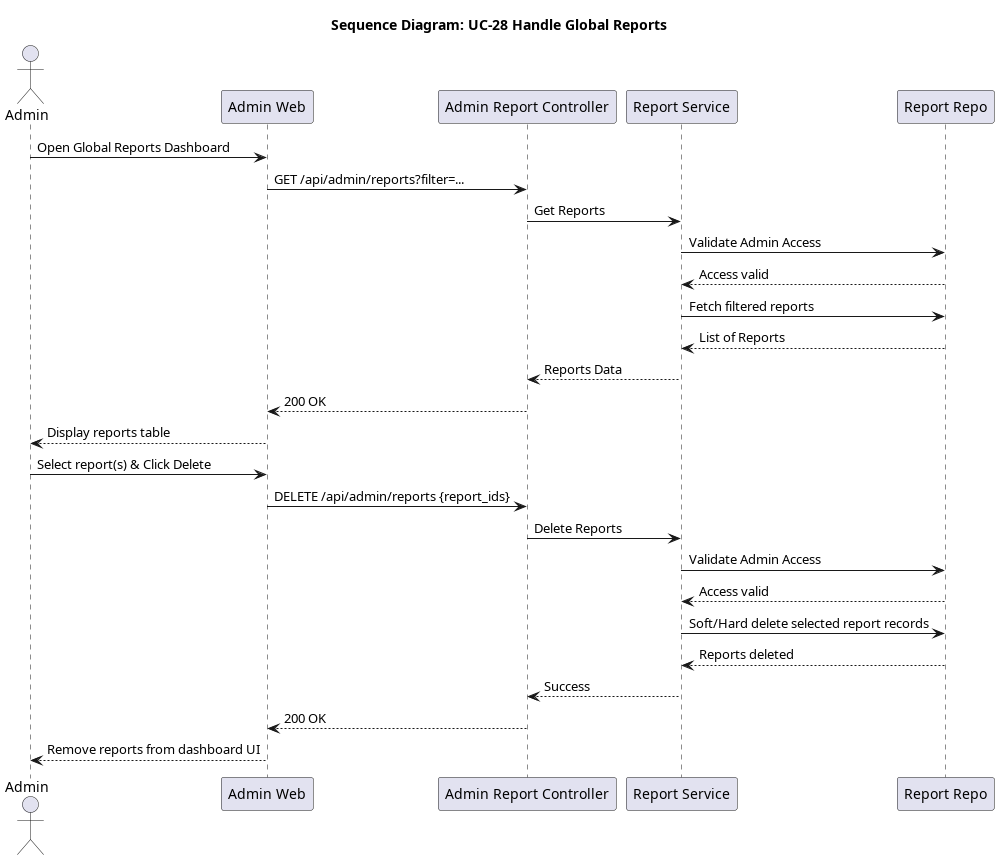
\includegraphics[width=0.9\textwidth]{diagrams/seq_28_handle_global_reports.png}
    \caption{Sequence Diagram for Handle Global Reports}
\end{figure}

\subsubsection{UC-29: Manage Platform}
\begin{figure}[H]
    \centering
    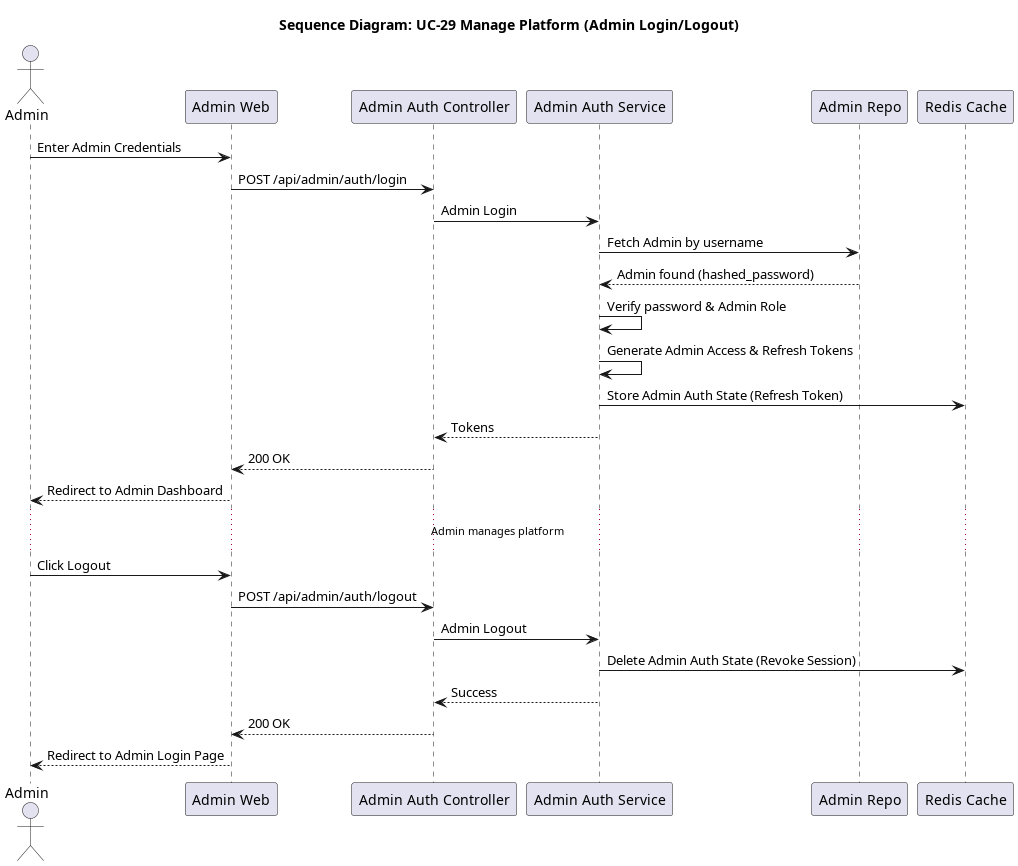
\includegraphics[width=0.9\textwidth]{diagrams/seq_29_manage_platform.png}
    \caption{Sequence Diagram for Manage Platform}
\end{figure}

\subsubsection{UC-30: View Analytics}
\begin{figure}[H]
    \centering
    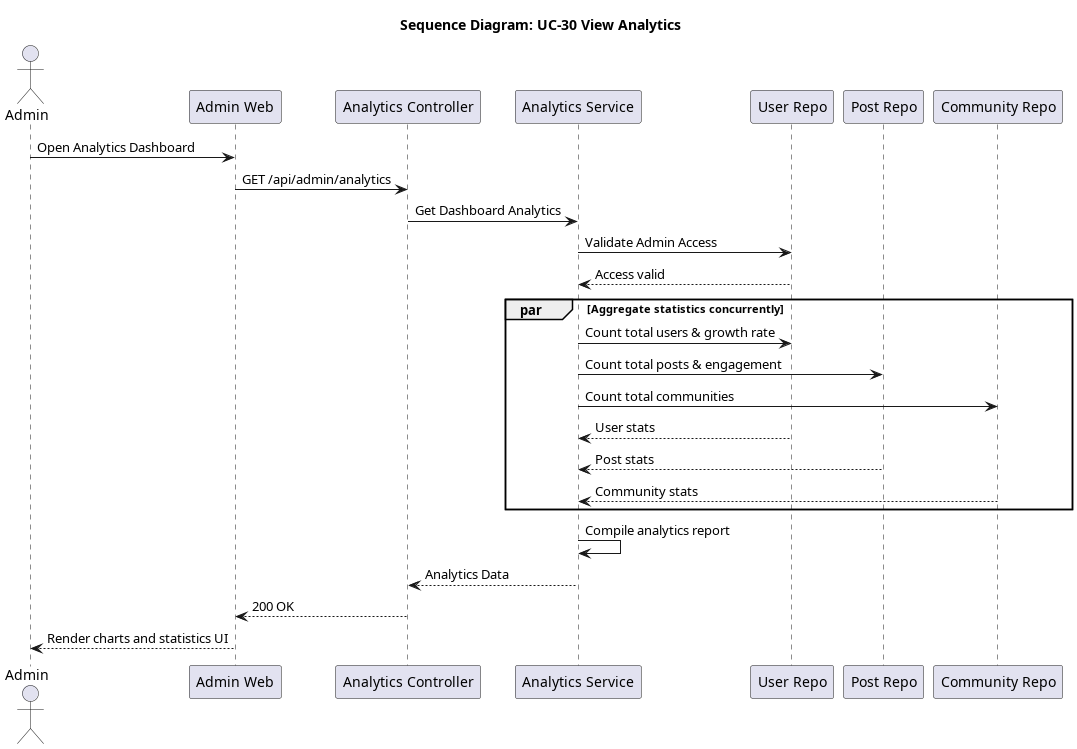
\includegraphics[width=0.9\textwidth]{diagrams/seq_30_view_analytics.png}
    \caption{Sequence Diagram for View Analytics}
\end{figure}

\section{Module View (Implementation Structure)}
This view defines how the codebase is structured logically, mapping to the \textbf{Component Diagram} in C4.

\subsection{Primary Presentation}
\begin{figure}[H]
    \centering
    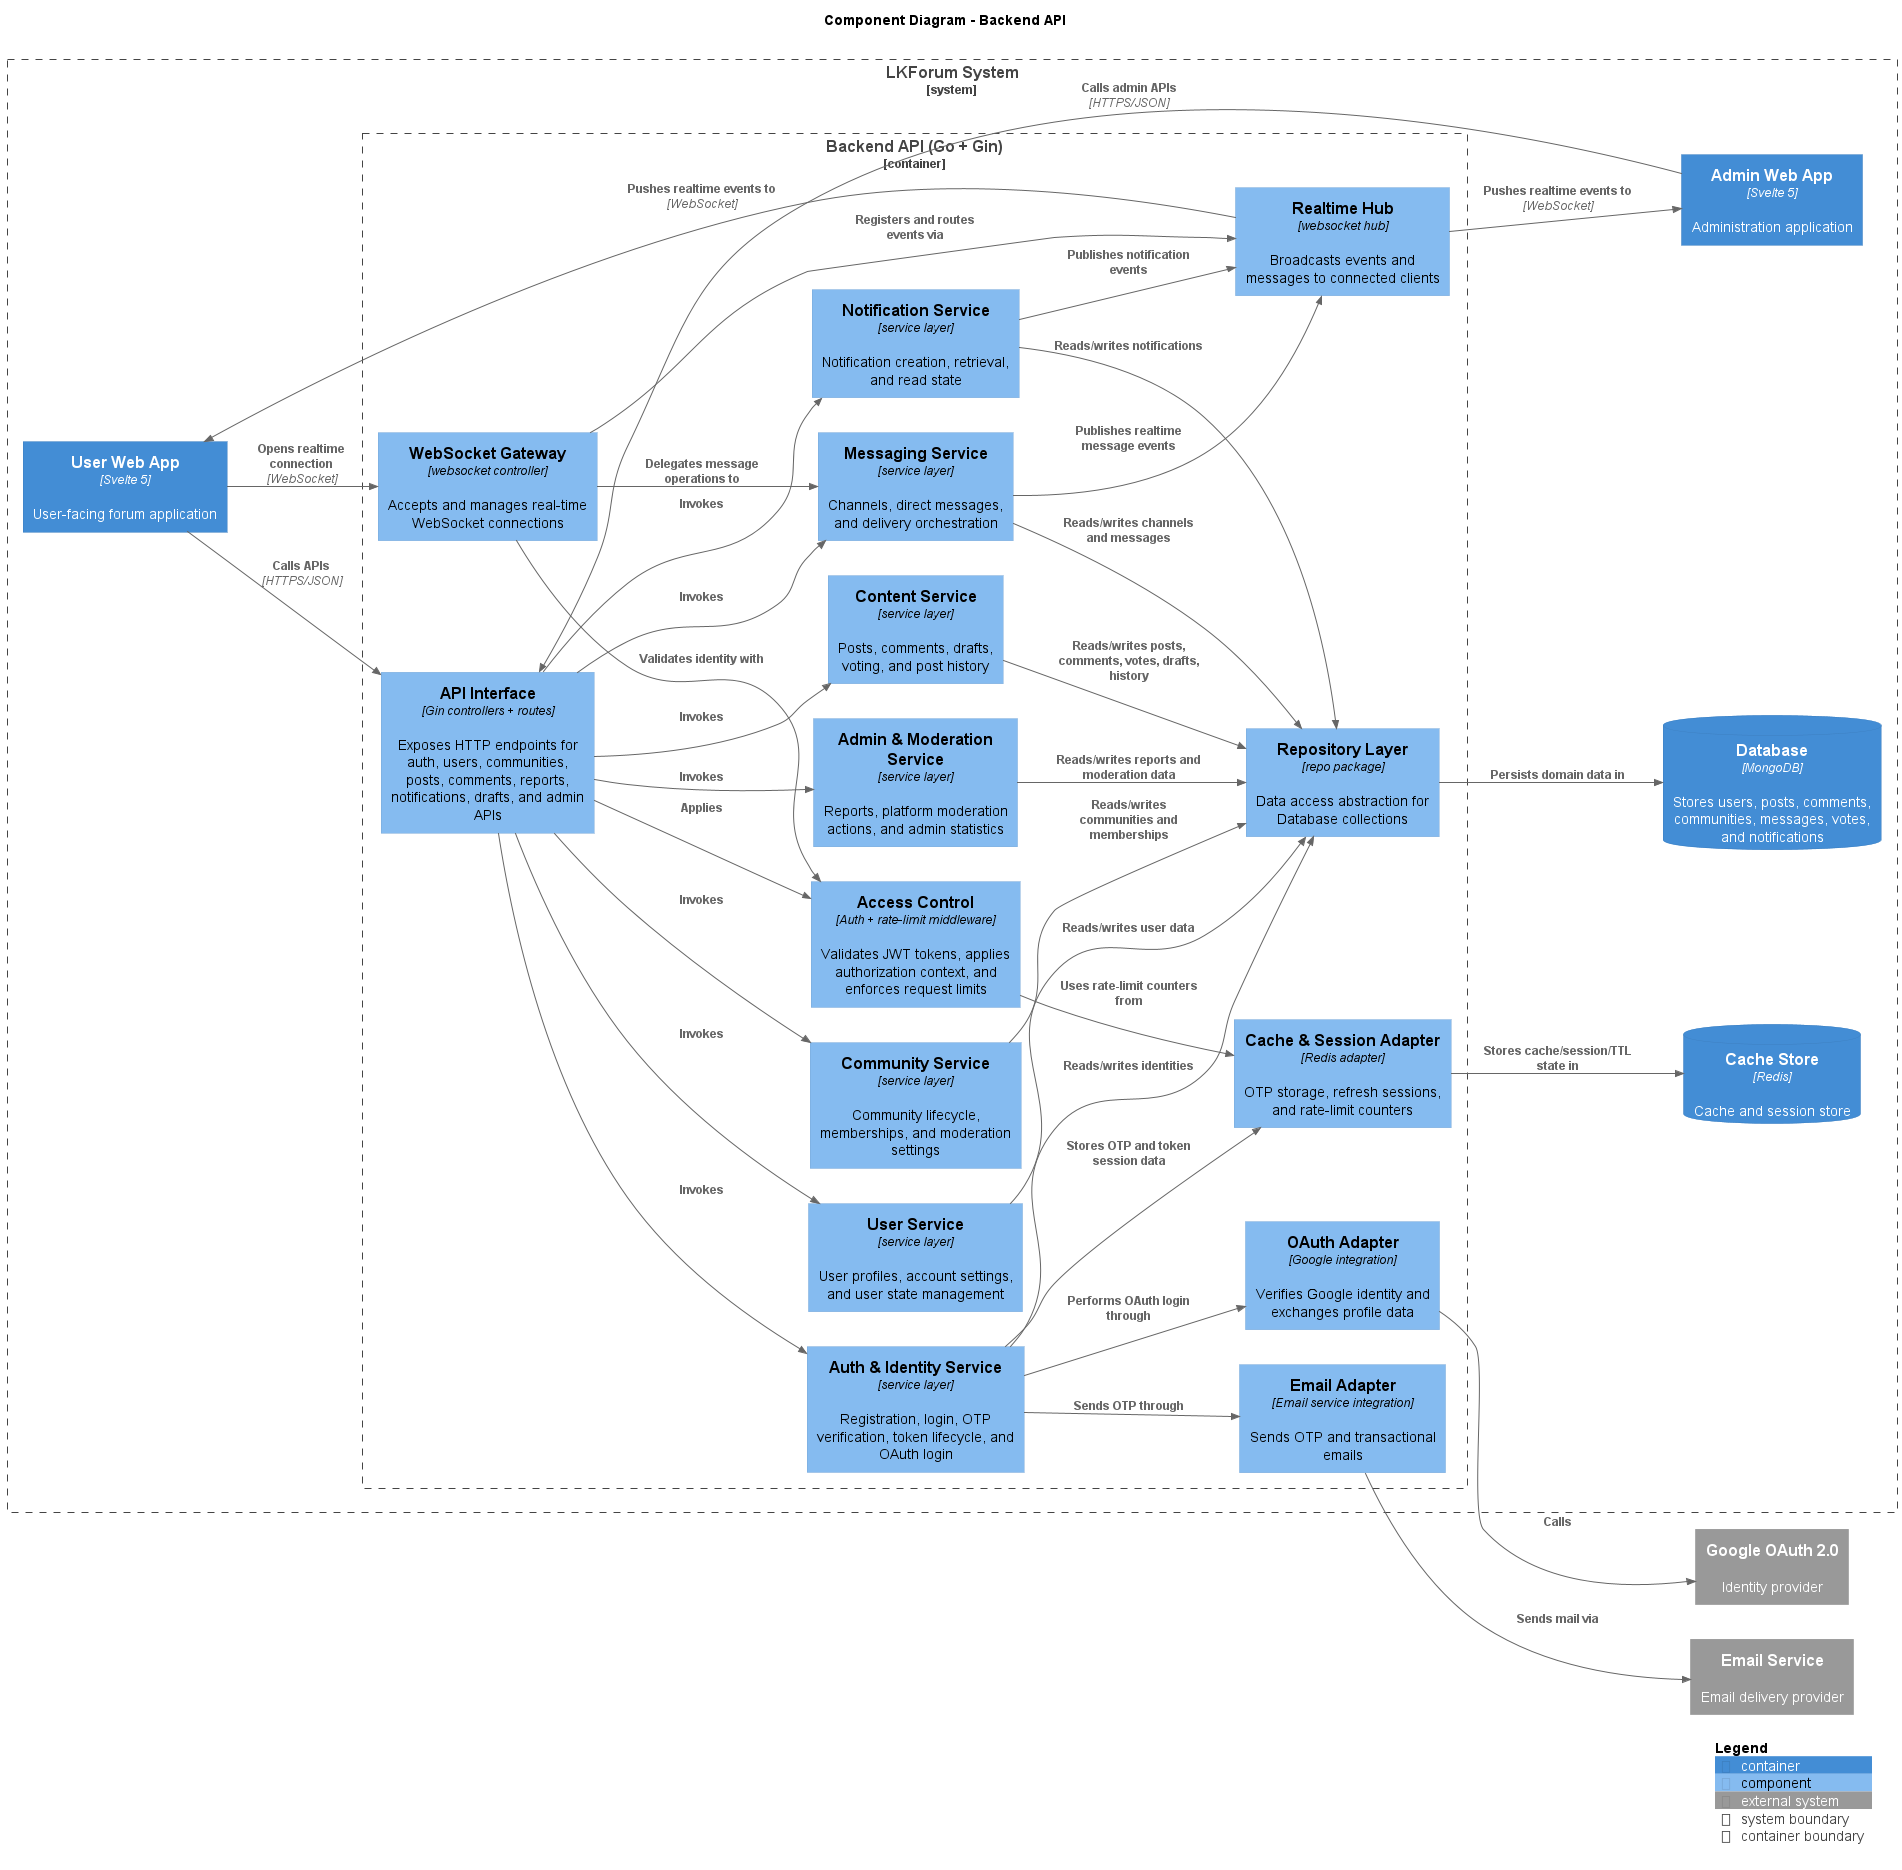
\includegraphics[width=0.9\textwidth]{c4/LKForum_Component_Backend.png}
    \caption{Backend Component Diagram}
\end{figure}

\subsection{Element Catalog}
\begin{itemize}
    \item \textbf{Routes \& Middlewares:} The entry point of the Go backend. It registers API endpoints and attaches global middlewares (such as JWT Validation, CORS handling, and structured Logging) before passing requests downstream.
    \item \textbf{Controllers (Handlers):} Responsible for parsing incoming HTTP requests (JSON/Multipart), validating input formats, and extracting parameters. Controllers do not contain business logic; they immediately delegate execution to the Service layer and format the HTTP responses.
    \item \textbf{Services (Business Logic):} The core of the application. Services contain all domain rules (e.g., verifying karma points, validating ownership, checking moderation states). They coordinate between Repositories, external systems, and the Event Bus.
    \item \textbf{Repositories (Data Access):} These modules abstract the database driver. They are responsible for constructing and executing MongoDB queries (BSON) and Redis commands, returning structured Go models to the Services.
    \item \textbf{Event Bus (Go Channels):} An internal communication mechanism. Services can publish events (e.g., \texttt{PostCreatedEvent}) to channels. Dedicated background goroutines listen to these channels to process asynchronous tasks like sending notifications, ensuring the main HTTP request is not blocked.
\end{itemize}

\section{Allocation View (Deployment)}
This view defines the mapping of software elements to the execution environments, aligning with the \textbf{Container Diagram} in C4.

\subsection{Primary Presentation}
\begin{figure}[H]
    \centering
    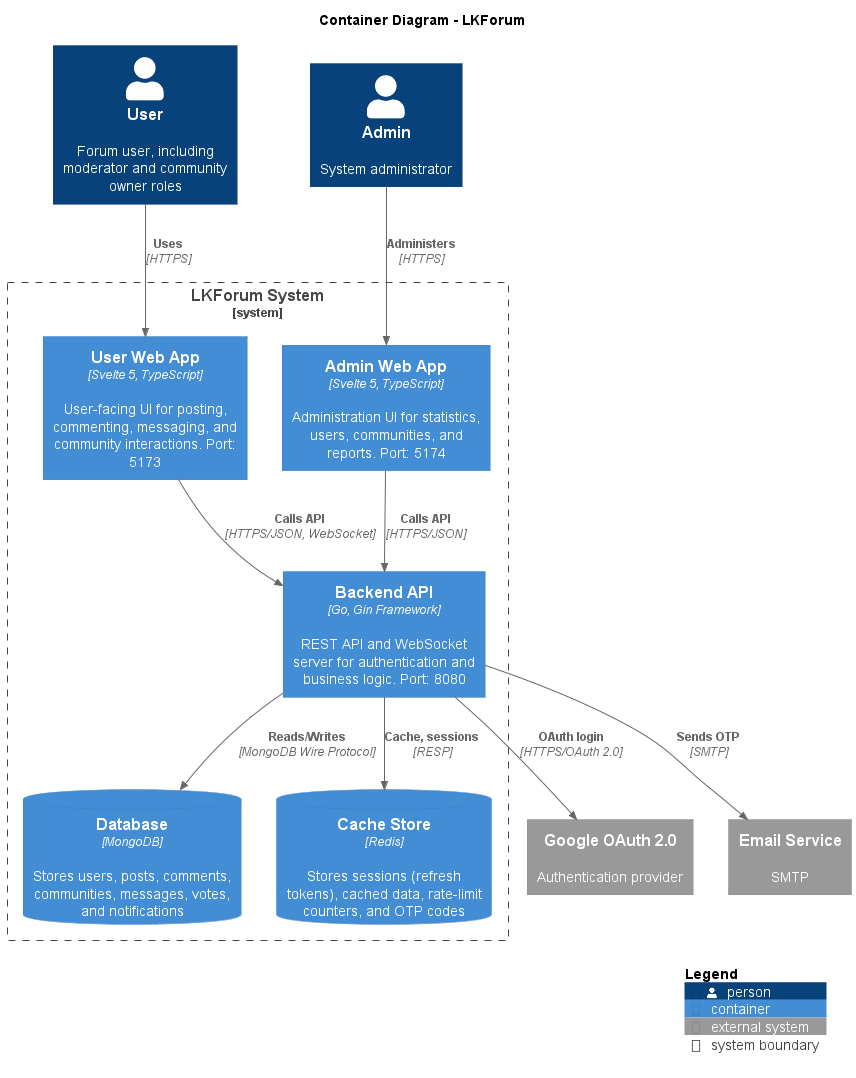
\includegraphics[width=0.9\textwidth]{c4/LKForum_Container.png}
    \caption{Container Diagram}
\end{figure}

\subsection{Element Catalog}
\begin{itemize}
    \item \textbf{Docker Compose (Environment):} Acts as the deployment orchestrator for a single-node setup. It defines the internal bridged network, container dependencies, and volume mounts.
    \item \textbf{User Web SPA Container:} A Node.js container serving the Svelte frontend application tailored for end-users. It communicates purely via REST APIs over HTTPS.
    \item \textbf{Admin Web SPA Container:} A separate Node.js container serving the isolated administrative dashboard. Physical separation ensures that administrative code is not delivered to standard users.
    \item \textbf{Go Backend API Container:} The compiled Go binary running inside a minimal Alpine or Scratch Linux image. It exposes port 8080 and handles all business transactions and WebSocket connections.
    \item \textbf{MongoDB Container:} The primary persistent data store running the NoSQL database engine. Data is stored in named Docker volumes to survive container restarts.
    \item \textbf{Redis Container:} The in-memory data structure store used for fast-expiring tokens, OTPs, and query result caching to reduce load on MongoDB.
    \item \textbf{Prometheus Container:} A time-series database configured to periodically scrape the \texttt{/metrics} endpoint of the Go Backend to record system health over time.
    \item \textbf{Grafana Container:} The observability dashboard. It connects to Prometheus to visualize system metrics and logs in real-time.
\end{itemize}

\chapter{Relations Among Views}
The views presented above are tightly interrelated. 
\begin{itemize}
    \item The external actors defined in the \textbf{System Context View} are the direct sources of the interactions detailed in the \textbf{Sequence Diagrams}.
    \item The structural layers described in the \textbf{Module View} (Controllers, Services, Repositories) map exactly to the participants (lifelines) executing the logic within each Sequence Diagram.
    \item Finally, the execution of the compiled codebase from the Module View requires the physical infrastructure defined in the \textbf{Allocation View}, where the Go codebase becomes a running container processing the requests originating from the SPA containers.
\end{itemize}

\end{document}
